\begin{enumerate}[label=\thesection.\arabic*,ref=\thesection.\theenumi]
\item The $4^{th}$ term of a G.P. is square of its second term, and the first term is -3. Determine its $7^{th}$ term.\\  

\solution 

\iffalse
\documentclass[journal,12pt,twocolumn]{IEEEtran}
\usepackage{amsmath,amssymb,amsfonts,amsthm}
\usepackage{txfonts}
\usepackage{tkz-euclide}
\usepackage{listings}
\usepackage{gvv}
\usepackage[latin1]{inputenc}
\usepackage{array}
\usepackage{pgf}
\usepackage{lmodern}

\begin{document}
\bibliographystyle{IEEEtran}

\title{DISCRETE 11.9.3 Q-4}
\author{EE23BTECH11066 - Yakkala Amarnath Karthik
}
\maketitle

\bibliographystyle{IEEEtran}
\textbf{Question:} \\ \\The $4^{th}$ term of a G.P. is square of its second term, and the first term is -3. Determine its $7^{th}$ term.\\ \\
\textbf{Solution:}
\fi
\begin{table}[h!]
  \centering
    \begin{tabular}{|c|c|c|}
    \hline
    \textbf{Variable} & \textbf{Description} & \textbf{value}\\
    \hline
    $x(0)$ & first term of G.P. & -3 \\
    \hline
    $r$ & Common ratio of G.P. & ? \\
    \hline
    $x(n)$ & general term of the G.P. & $x\brak0r^{n}$ \\
    \hline
    $x\brak3$ & fourth term & $\sbrak{x\brak1}^2$\\
    \hline
    $u\brak{n}$ & unit step function & - \\
    \hline
  \end{tabular}

  \caption{A Table with input parameters}
  \label{tab:11.9.3.4.1}
\end{table}
from \tabref{tab:11.9.3.4.1}
\begin{align}
 x\brak0r^{3}&=\brak{x\brak0r^{1}}^2\\
 &=x\brak0^2r^2\\
\implies r&=x\brak0\\
&=-3
\end{align}
general term
\begin{align}
x\brak{n}&=x\brak0r^nu\brak{n}\\
&=\brak{-3}^{n+1}u\brak{n}
\end{align}
The $7^{th}$ term of the sequence will be:
\begin{align}
x\brak6 & =\brak{-3}\brak{-3}^{6}\\
& =-2187
\end{align}
Z transform of the given G.P is:
\begin{align}
X\brak{z}=\frac{x\brak0}{1-rz^{-1}}= \frac{-3}{1+3z^{-1}}.\hspace{0.5cm} |z|>3
\end{align}
\bigskip
\begin{figure}[ht]
        \centering
        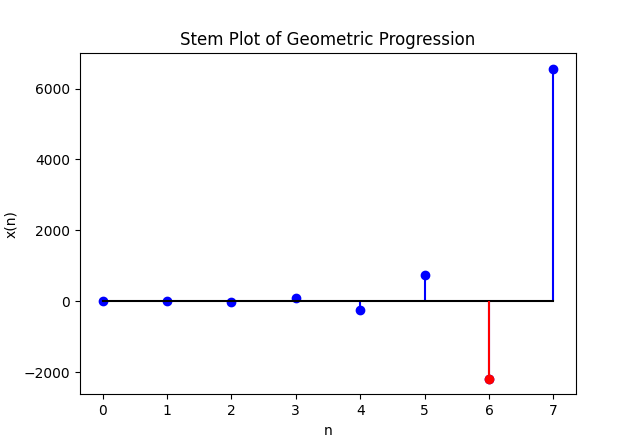
\includegraphics[width=0.45\textwidth]{ncert-maths/11/9/3/4/figs/stemplotfinal.jpeg}
        \caption{Graph showing first 8 terms of the GP}
    \end{figure} \\
%\end{document}

\pagebreak

\item Show that
\begin{equation}
    \frac{1\times2^2 + 2\times3^2 + \dots + n\times\brak{n+1}^2}{1^2\times2 + 2^2\times3 +\dots + n^2\times\brak{n+1}}  = \frac{3n+5}{3n+1}\notag
\end{equation}

\solution 

\iffalse
\let\negmedspace\undefined
\let\negthickspace\undefined
\documentclass[journal,12pt,twocolumn]{IEEEtran}
\usepackage{cite}
\usepackage{amsmath,enumitem,amssymb,amsfonts,amsthm}
\usepackage{algorithmic}
\usepackage{graphicx}
\usepackage{float}
\usepackage{textcomp}
\usepackage{xcolor}
\usepackage{caption}
\usepackage{txfonts}
\usepackage{listings}
\usepackage{enumitem}
\usepackage{mathtools}
\usepackage{gensymb}
\usepackage{comment}
\usepackage[breaklinks=true]{hyperref} 
\usepackage{tkz-euclide} 
\usepackage{listings}
\usepackage{tabularx}
\usepackage{gvv}                                        
\def\inputGnumericTable{}                                 
\usepackage[latin1]{inputenc}                              
\usepackage{color}                                            
\usepackage{array}                                            
\usepackage{longtable}                                       
\usepackage{calc}                                             
\usepackage{multirow}                                         
\usepackage{hhline}                                           
\usepackage{ifthen}                                        
\usepackage{lscape}
\newtheorem{theorem}{Theorem}[section]
\newtheorem{problem}{Problem}
\newtheorem{proposition}{Proposition}[section]
\newtheorem{lemma}{Lemma}[section]
\newtheorem{corollary}[theorem]{Corollary}
\newtheorem{example}{Example}[section]
\newtheorem{definition}[problem]{Definition}
\newcommand{\BEQA}{\begin{eqnarray}}
\newcommand{\EEQA}{\end{eqnarray}}
\newcommand{\define}{\stackrel{\triangle}{=}}
\theoremstyle{remark}
\newtheorem{rem}{Remark}
\begin{document}
\bibliographystyle{IEEEtran}
\vspace{3cm}
\title{NCERT 11.9.5 26Q}
\author{EE23BTECH11015 - DHANUSH V NAYAK$^{*}$% <-this % stops a space
}
\maketitle
\newpage
\bigskip
\renewcommand{\thefigure}{\arabic{figure}}
\renewcommand{\thetable}{\theenumi}
\bibliographystyle{IEEEtran}
\textbf{\underline{RESULTS AND DERIVATIONS}}

\newpage
\textbf{Question:} Show that
\begin{equation}
    \frac{1\times2^2 + 2\times3^2 + \dots + n\times\brak{n+1}^2}{1^2\times2 + 2^2\times3 +\dots + n^2\times\brak{n+1}}  = \frac{3n+5}{3n+1}\notag
\end{equation}
\textbf{Solution:}
\fi 

\begin{table}[h]
    \centering
    \renewcommand\thetable{1}
    \setlength{\extrarowheight}{9pt}
    \resizebox{0.54\textwidth}{!}{
    \begin{tabular}{|c|c|c|}
    \hline
    \textbf{Parameter} & \textbf{Description} & \textbf{Value} \\ \hline
    $n$ & Integer &.... -2,-1,0,1, 2, ... \\ \hline
    $x_1(n)$ & General term of Numerator & $\vphantom{\brak{n^{3}}} \brak{n^{3} + 5n^{2} + 8n + 4} \cdot u\brak{n}$ \\ \hline
    $x_2(n)$ & General Term of Denominator  & $\vphantom{\brak{n^{3}}} \brak{n^{3}+4n^{2}+5n+2}\cdot u\brak{n}$ \\ \hline
    $y_1\brak{n}$ & Sum of terms of numerator & $?$ \\ \hline
    $y_2\brak{n}$ & Sum of terms of denominator & $? $ \\ \hline
    $U(z)$ & z-transform of $u(n)$ & $\frac{1}{1 - z^{-1}\vphantom {\brak{0.3pt}}},\cbrak{z\in\mathbb{C} : \lvert z \rvert > 1}$ \\ \hline 
    ROC & Region of convergence & $\left\{ z : \left|\sum_{n=-\infty}^{\infty} x(n)z^{-n}\right| < \infty \vphantom {\brak{{0.3pt}}}\right\}$ \\ \hline 
    \end{tabular}}
    \caption{Parameter Table}
    \label{tab:11.9.5.26.1}
    \end{table}
    
    
    
    
\begin{enumerate}[label=\arabic*.]
\item \underline {Analysis of Numerator:}\\
\begin{align}
 X_1\brak{z} &= \sum_{n=-\infty}^\infty x_1\brak{n}  z^{-n}\\
             &= \sum_{n=-\infty}^\infty \brak{n^{3} + 5n^{2} + 8n + 4} u\brak{n} z^{-n}
\end{align}
Using results of equations \eqref{eq:11.9.5.26.2} to \eqref{eq:11.9.5.26.5} we get:
\begin{align}
 \therefore   X_1\brak{z}&= \frac{4+2z^{-1}}{\brak{1-z^{-1}}^4} ,   \abs{z} >1 
\end{align}
From \eqref{eq:conv-sum}
\begin{align}
y_1\brak{n} &= x_1\brak{n}\ast u\brak{n}\\
    Y_1\brak{z} &= X_1\brak{z} U\brak{z} \\
 &= \frac{4+2z^{-1}}{\brak{1-z^{-1}}^5} , \abs{z}> 1 
\end{align}
Using partial fractions:
\begin{align}
    Y_1(z) &= \frac{22z^{-1}}{\brak{1-z^{-1}}} + \frac{48z^{-2}}{\brak{1-z^{-1}}^2} + \frac{52z^{-3}}{\brak{1-z^{-3}}^3} , \label{eq:11.9.5.26.6}\\
    &+ \frac{28z^{-4}}{\brak{1-z^{-1}}^4}+\frac{6z^{-5}}{\brak{1-z^{-1}}^5}+4 , \abs{z}>1 \notag 
\end{align}
Substituting results of equation \eqref{eq:11.9.5.26.9} to \eqref{eq:11.9.5.26.12} in equation \eqref{eq:11.9.5.26.6}:
\begin{align}
    y_1\brak{n} &= \frac{3n^4 + 26n^3 + 81n^2 + 106n + 48}{12}u\brak{n}\\
    &= \frac{\brak{3n+8}\brak{n+1}\brak{n+2}\brak{n+3}}{12}u\brak{n}
\end{align}
\item \underline{Analysis of Denominator:}
\begin{align}
    X_2\brak{z} &= \sum_{n=-\infty}^\infty x_2\brak{n} z^{-n}\\
                &= \sum_{n=-\infty}^\infty \brak{n^{3}+4n^{2}+5n+2} u\brak{n} z^{-n}
\end{align}
\text{Using results of equation \eqref{eq:11.9.5.26.2} to \eqref{eq:11.9.5.26.5} we get:}
\begin{align}
   \therefore  X_2\brak{z} &= \frac{2+4z^{-1}}{\brak{1-z^{-1}}^4},   \abs{z} >1   
\end{align}
From \eqref{eq:conv-sum}
\begin{align}
    y_2\brak{n} &= x_2\brak{n}\ast u\brak{n}\\
    Y_2\brak{z} &= X_2\brak{z} U\brak{z} \\
 &=\frac{2+4z^{-1}}{\brak{1-z^{-1}}^5} ,   \abs{z} >1 
\end{align}
Using partial fractions:
\begin{align}
    Y_2\brak{z} &= \frac{14z^{-1}}{\brak{1-z^{-1}}} + \frac{36z^{-2}}{\brak{1-z^{-1}}^2} + \frac{44z^{-3}}{\brak{1-z^{-3}}^3} \label{eq:11.9.5.26.13}\\
    &+ \frac{26z^{-4}}{\brak{1-z^{-1}}^4}+\frac{6z^{-5}}{\brak{1-z^{-1}}^5}+2 , \abs{z}>1\notag 
\end{align}
Substituting results of equation \eqref{eq:11.9.5.26.9} to \eqref{eq:11.9.5.26.12} in equation \eqref{eq:11.9.5.26.13}:
\begin{align}
    y_2\brak{n} &=  \frac{3n^4 + 22n^3 + 57n^2 + 62n + 24}{12}u\brak{n}\\
                &= \frac{\brak{3n+4}\brak{n+1}\brak{n+2}\brak{n+3}}{12}u\brak{n}
\end{align}
As the sequence start from $n=0$ , in RHS of question $n$ should be replaced by $n+1$:
\begin{align}
    \frac{y_1\brak{n}}{y_2\brak{n}} = \frac{3n+8}{3n+4}
\end{align}
Hence Prooved.
\end{enumerate}
\begin{figure}[htbp]
    \centering
    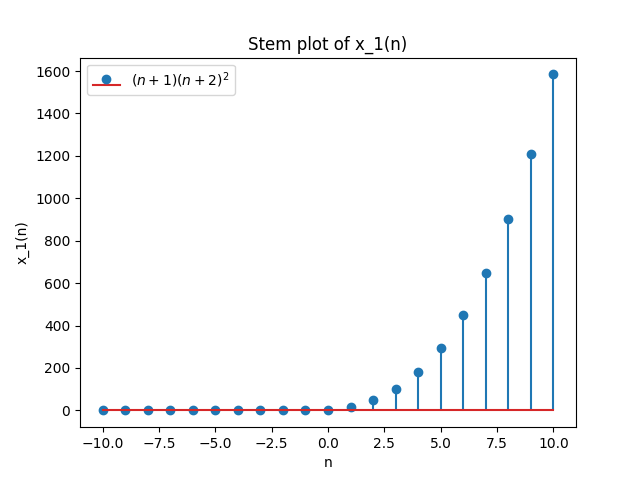
\includegraphics[width=1\columnwidth]{ncert-maths/11/9/5/26/figs/x1_plot.png}
    \caption{Stem Plot of $x_1\brak{n}$}
    \label{fig:x1}
\end{figure}
\begin{figure}[htbp]
    \centering
    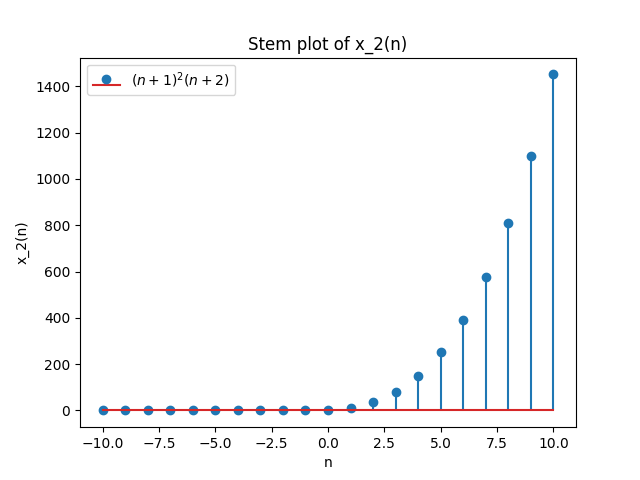
\includegraphics[width=1\columnwidth]{ncert-maths/11/9/5/26/figs/x2_plot.png}
    \caption{Stem Plot of $x_2\brak{n}$}
    \label{fig:x2}
\end{figure}
\begin{figure}[htbp]
    \centering
    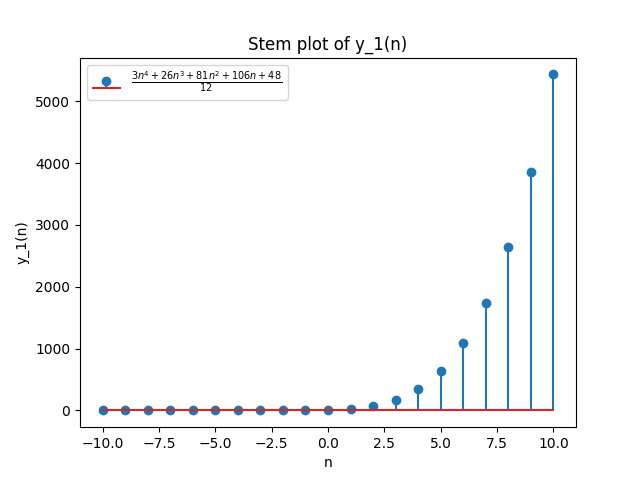
\includegraphics[width=1\columnwidth]{ncert-maths/11/9/5/26/figs/y1_plot.png}
    \caption{Stem Plot of $y_1\brak{n}$}
    \label{fig:y1}
\end{figure}
\begin{figure}[h]
    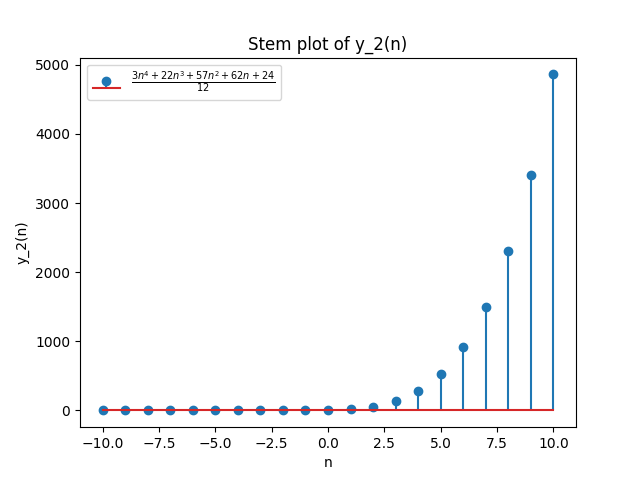
\includegraphics[width=1\columnwidth]{ncert-maths/11/9/5/26/figs/y2_plot.png}
    \caption{Stem Plot of $y_2\brak{n}$}
    \label{fig:y2}
\end{figure}
%\end{document}

\pagebreak

\item Write the five terms at n = 1, 2, 3, 4, 5 of the sequence and obtain the Z-transform of the series
\begin{align}
    x \brak{n} &=  -1, & n = 0 \\
    &=   \frac{x \brak{n-1}}{n}, & n > 0\\
    &=   0, & n < 0 
\end{align}

\solution

\iffalse
\let\negmedspace\undefined
\let\negthickspace\undefined
\documentclass[journal,12pt,twocolumn]{IEEEtran}
\usepackage{cite}
\usepackage{amsmath,amssymb,amsfonts}
\usepackage{graphicx}
\usepackage{textcomp}
\usepackage{xcolor}
\usepackage{txfonts}
\usepackage{listings}
\usepackage{enumitem}
\usepackage{mathtools}
\usepackage{gensymb}
\usepackage{comment}
\usepackage[breaklinks=true]{hyperref}
\usepackage{tkz-euclide} 
\usepackage{listings}
\usepackage{gvv}                                        
\def\inputGnumericTable{}                                 
\usepackage[latin1]{inputenc}                                
\usepackage{color}                                            
\usepackage{array}                                            
\usepackage{longtable}                                       
\usepackage{calc}                                             
\usepackage{multirow}                                         
\usepackage{hhline}                                           
\usepackage{ifthen}                                           
\usepackage{lscape}
\usepackage[export]{adjustbox}

\newtheorem{theorem}{Theorem}[section]
\newtheorem{problem}{Problem}
\newtheorem{proposition}{Proposition}[section]
\newtheorem{lemma}{Lemma}[section]
\newtheorem{corollary}[theorem]{Corollary}
\newtheorem{example}{Example}[section]
\newtheorem{definition}[problem]{Definition}
\newcommand{\BEQA}{\begin{eqnarray}}
\newcommand{\EEQA}{\end{eqnarray}}
\newcommand{\define}{\stackrel{\triangle}{=}}
\newtheorem{rem}{Remark}

\begin{document}
\parindent 0px
\bibliographystyle{IEEEtran}

\vspace{3cm}

\title{}
\author{EE23BTECH11217 - Prajwal M$^{*}$
}
\maketitle
\newpage
\bigskip

 \renewcommand{\thefigure}{\theenumi}
 \renewcommand{\thetable}{\theenumi}


\section*{Exercise 9.1}

\noindent \textbf{12} \hspace{2pt}Write the five terms at n = 1, 2, 3, 4, 5 of the sequence and obtain the Z-transform of the series
\begin{align}
    x \brak{n} &=  -1, & n = 0 \\
    &=   \frac{x \brak{n-1}}{n}, & n > 0\\
    &=   0, & n < 0 
\end{align}

\noindent Solution:
\fi
\noindent
\begin{align}
	x \brak{1} & = \frac{x \brak{0}}{1} = -1 \\
x \brak{2} & = \frac{x \brak{1}}{2} = -\frac{1}{2} \\
	x \brak{3} & = \frac{x \brak{2}}{3} = -\frac{1}{\brak{2} \brak{3}} = -\frac{1}{6}\\
	x \brak{4} & = \frac{x \brak{3}}{4} = -\frac{1}{\brak{2}   \brak{3} \brak{4}} = -\frac{1}{24}\\
	x \brak{5} & = \frac{x \brak{4}}{5} = -\frac{1}{\brak{2} \brak{3} \brak{4} \brak{5}} = -\frac{1}{120} \\
    x \brak{n} & = \frac{-1}{n!}  \brak{u \brak{n}} \label{x(n)}
\end{align}
\begin{align}
	x \brak{n} & \system{Z} X \brak{z} 
\end{align}

\begin{figure}[h]
   \centering
   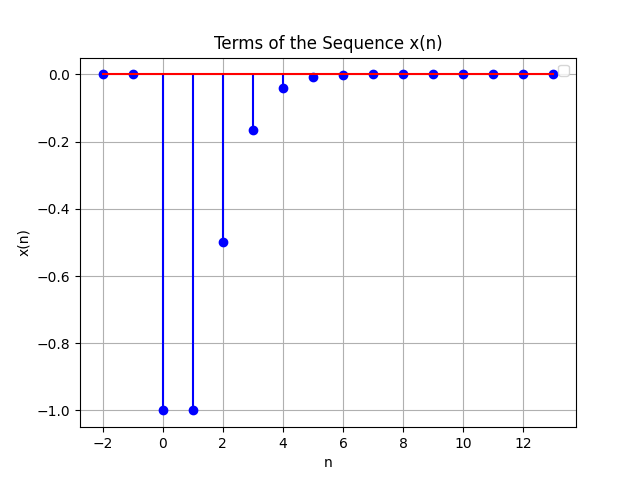
\includegraphics[width=1\columnwidth]{ncert-maths/11/9/1/12/figs/plot.png}
   \caption{Plot of x(n) vs n}
   \label{fig: 9.1.12.1}
\end{figure}

\begin{align}
    X \brak{z} & = \sum_{n=-\infty}^{\infty} x \brak{n}   z^{-n} \\
    \notag \text{using \eqref{x(n)}, } \\
    & = \sum_{n=-\infty}^{\infty} \frac{-1}{n!}  u \brak{n}   z^{-n} \\
    & = \sum_{n=0}^{\infty} \frac{-1}{n!}   z^{-n} \\
    & = - e^{z^{-1}} &  \cbrak{z\in\mathbb{C} : z \neq 0} 
\end{align}

\begin{table}[h]
    \centering
      \begin{tabular}{|c|c|c|}
    \hline
    	\textbf{Symbol} & \textbf{Value} & \textbf{Description} \\
    \hline
	  $x(n)$ & $\frac{-1}{n!}$ & general term of the series \\
    \hline
	  $X(z)$ & $- e^{z^{-1}}$ &Z-transform of x(n) \\
    \hline 
	  $u(n)$ & &unit step function \\
    \hline
  \end{tabular}

    \caption{Parameters}
    \label{tab: 9.1.12.1}
\end{table}


%\end{document}

\pagebreak


\item Subba Rao started work in 1995 at an annual salary of Rs. 5000 and received an increment of Rs. 200 each year. In which year did his income reach Rs. 7000?

\solution

\iffalse
\let\negmedspace\undefined
\let\negthickspace\undefined
\documentclass[journal,12pt,twocolumn]{IEEEtran}
\usepackage{cite}
\usepackage{amsmath,amssymb,amsfonts,amsthm}
\usepackage{algorithmic}
\usepackage{graphicx}
\usepackage{textcomp}
\usepackage{xcolor}
\usepackage{txfonts}
\usepackage{listings}
\usepackage{enumitem}
\usepackage{mathtools}
\usepackage{gensymb}
\usepackage{comment}
\usepackage[breaklinks=true]{hyperref}
\usepackage{tkz-euclide}
\usepackage{listings}
\usepackage{gvv}
\def\inputGnumericTable{}
\usepackage[latin1]{inputenc}
\usepackage{color}
\usepackage{array}
\usepackage{longtable}
\usepackage{calc}
\usepackage{multirow}
\usepackage{hhline}
\usepackage{ifthen}
\usepackage{lscape}

\newtheorem{theorem}{Theorem}[section]
\newtheorem{problem}{Problem}
\newtheorem{proposition}{Proposition}[section]
\newtheorem{lemma}{Lemma}[section]
\newtheorem{corollary}[theorem]{Corollary}
\newtheorem{example}{Example}[section]
\newtheorem{definition}[problem]{Definition}
\newcommand{\BEQA}{\begin{eqnarray}}
\newcommand{\EEQA}{\end{eqnarray}}
\newcommand{\define}{\stackrel{\triangle}{=}}
\theoremstyle{remark}
\newtheorem{rem}{Remark}
\begin{document}

\bibliographystyle{IEEEtran}
\vspace{3cm}

\title{NCERT Discrete - 10.5.2.19}
\author{EE23BTECH11007 - Aneesh Kadiyala$^{*}$% <-this % stops a space
}
\maketitle
\newpage
\bigskip

\renewcommand{\thefigure}{\theenumi}
\renewcommand{\thetable}{\theenumi}
\vspace{3cm}
\textbf{Question 10.5.2.19:} Subba Rao started work in 1995 at an annual salary of Rs. 5000 and received an increment of Rs. 200 each year. In which year did his income reach Rs. 7000?

\solution
\fi
\begin{table}[h!]
    \centering
    \begin{tabular}{ | c | c | c | }
        \hline
        Parameter & Value & Description \\
        \hline
        $x(0)$ & 5000 & Initial Income \\
        \hline
        $d$ & 200 & Annual Increment (Common Difference) \\
        \hline
        $x(n)$ & $(x(0) + nd)u(n)$ & $n^{th}$ term of the AP \\
        \hline
    \end{tabular}
    \caption{Input Parameters}
    \label{tab:math_10_5_2_19}
\end{table}
From the values given in \tabref{tab:math_10_5_2_19}:
\begin{align}
7000 &= 5000 + 200n \\
\implies 2000 &= 200n \\
\therefore n &= 10
\end{align}
\begin{figure}[h!]
    \centering
    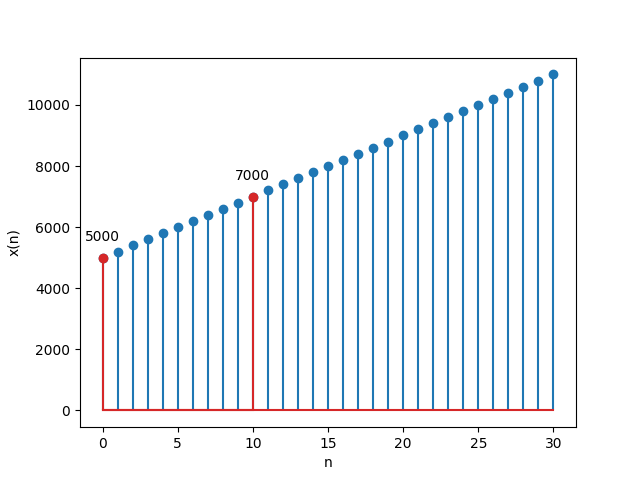
\includegraphics[width=\columnwidth]{ncert-maths/10/5/2/19/figs/10_5_2_19.png}
    \caption{Plot of $x(n)$ vs $n$. See \tabref{tab:math_10_5_2_19} for details.}
    \label{fig:math_10_5_2_19}
\end{figure}
Let Z-transform of $x(n)$ be $X(z)$.
\begin{align}
X(z) &= \frac{x(0)}{1 - z^{-1}} + \frac{dz^{-1}}{(1 - z^{-1})^2} \quad |z| > 1
\end{align}
Using the values from \tabref{tab:math_10_5_2_19}:
\begin{align}
X(z) &= \frac{5000}{1 - z^{-1}} + \frac{200z^{-1}}{(1 - z^{-1})^2} \quad |z| > 1
\end{align}
%\end{document}


\item Consider the sequence whose $n^\text{th}$ term is given by \(2^n\). Find the first 6 terms of this sequence.

\solution

%\iffalse
\let\negmedspace\undefined
\let\negthickspace\undefined
\documentclass[journal,12pt,onecolumn]{IEEEtran}
\usepackage{cite}
\usepackage{amsmath,amssymb,amsfonts,amsthm}
%\usepackage{algorithmic}
\usepackage{graphicx}
\usepackage{textcomp}
\usepackage{array}
\usepackage{xcolor}
\usepackage{txfonts}
\usepackage{listings}
\usepackage{enumitem}
\usepackage{mathtools}
\usepackage{gensymb}
\usepackage[breaklinks=true]{hyperref}
\usepackage{tkz-euclide} % loads  TikZ and tkz-base
\usepackage{listings}
\usepackage{float}



\newtheorem{theorem}{Theorem}[section]
\newtheorem{problem}{Problem}
\newtheorem{proposition}{Proposition}[section]
\newtheorem{lemma}{Lemma}[section]
\newtheorem{corollary}[theorem]{Corollary}
\newtheorem{example}{Example}[section]
\newtheorem{definition}[problem]{Definition}
%\newtheorem{thm}{Theorem}[section] 
%\newtheorem{defn}[thm]{Definition}
%\newtheorem{algorithm}{Algorithm}[section]
%\newtheorem{cor}{Corollary}
\newcommand{\BEQA}{\begin{eqnarray}}
\newcommand{\EEQA}{\end{eqnarray}}
\newcommand{\define}{\stackrel{\triangle}{=}}
\theoremstyle{remark}
\newtheorem{rem}{Remark}
%\bibliographystyle{ieeetr}
\begin{document}
%
\providecommand{\pr}[1]{\ensuremath{\Pr\left(#1\right)}}
\providecommand{\prt}[2]{\ensuremath{p_{#1}^{\left(#2\right)} }}        % own macro for this question
\providecommand{\qfunc}[1]{\ensuremath{Q\left(#1\right)}}
\providecommand{\sbrak}[1]{\ensuremath{{}\left[#1\right]}}
\providecommand{\lsbrak}[1]{\ensuremath{{}\left[#1\right.}}
\providecommand{\rsbrak}[1]{\ensuremath{{}\left.#1\right]}}
\providecommand{\brak}[1]{\ensuremath{\left(#1\right)}}
\providecommand{\lbrak}[1]{\ensuremath{\left(#1\right.}}
\providecommand{\rbrak}[1]{\ensuremath{\left.#1\right)}}
\providecommand{\cbrak}[1]{\ensuremath{\left\{#1\right\}}}
\providecommand{\lcbrak}[1]{\ensuremath{\left\{#1\right.}}
\providecommand{\rcbrak}[1]{\ensuremath{\left.#1\right\}}}
\newcommand{\sgn}{\mathop{\mathrm{sgn}}}
\providecommand{\abs}[1]{\left\vert#1\right\vert}
\providecommand{\res}[1]{\Res\displaylimits_{#1}} 
\providecommand{\norm}[1]{\left\lVert#1\right\rVert}
%\providecommand{\norm}[1]{\lVert#1\rVert}
\providecommand{\mtx}[1]{\mathbf{#1}}
\providecommand{\mean}[1]{E\left[ #1 \right]}
\providecommand{\cond}[2]{#1\middle|#2}
\providecommand{\fourier}{\overset{\mathcal{F}}{ \rightleftharpoons}}
\newenvironment{amatrix}[1]{%
  \left(\begin{array}{@{}*{#1}{c}|c@{}}
}{%
  \end{array}\right)
}
%\providecommand{\hilbert}{\overset{\mathcal{H}}{ \rightleftharpoons}}
%\providecommand{\system}{\overset{\mathcal{H}}{ \longleftrightarrow}}
	%\newcommand{\solution}[2]{\textbf{Solution:}{#1}}
\newcommand{\solution}{\noindent \textbf{Solution: }}
\newcommand{\cosec}{\,\text{cosec}\,}
\providecommand{\dec}[2]{\ensuremath{\overset{#1}{\underset{#2}{\gtrless}}}}
\newcommand{\myvec}[1]{\ensuremath{\begin{pmatrix}#1\end{pmatrix}}}
\newcommand{\mydet}[1]{\ensuremath{\begin{vmatrix}#1\end{vmatrix}}}
\newcommand{\myaugvec}[2]{\ensuremath{\begin{amatrix}{#1}#2\end{amatrix}}}
\providecommand{\rank}{\text{rank}}
\providecommand{\pr}[1]{\ensuremath{\Pr\left(#1\right)}}
\providecommand{\qfunc}[1]{\ensuremath{Q\left(#1\right)}}
	\newcommand*{\permcomb}[4][0mu]{{{}^{#3}\mkern#1#2_{#4}}}
\newcommand*{\perm}[1][-3mu]{\permcomb[#1]{P}}
\newcommand*{\comb}[1][-1mu]{\permcomb[#1]{C}}
\providecommand{\qfunc}[1]{\ensuremath{Q\left(#1\right)}}
\providecommand{\gauss}[2]{\mathcal{N}\ensuremath{\left(#1,#2\right)}}
\providecommand{\diff}[2]{\ensuremath{\frac{d{#1}}{d{#2}}}}
\providecommand{\myceil}[1]{\left \lceil #1 \right \rceil }
\newcommand\figref{Fig.~\ref}
\newcommand\tabref{Table~\ref}
\newcommand{\sinc}{\,\text{sinc}\,}
\newcommand{\rect}{\,\text{rect}\,}
%%
%	%\newcommand{\solution}[2]{\textbf{Solution:}{#1}}
%\newcommand{\solution}{\noindent \textbf{Solution: }}
%\newcommand{\cosec}{\,\text{cosec}\,}
%\numberwithin{equation}{section}
%\numberwithin{equation}{subsection}
%\numberwithin{problem}{section}
%\numberwithin{definition}{section}
%\makeatletter
%\@addtoreset{figure}{problem}
%\makeatother

%\let\StandardTheFigure\thefigure
\let\vec\mathbf

\bibliographystyle{IEEEtran}





\bigskip

%\renewcommand{\thefigure}{\theenumi}
%\renewcommand{\thetable}{\theenumi}
%\renewcommand{\theequation}{\theenumi}

Q: Consider the sequence whose $n^\text{th}$ term is given by \(2^n\). Find the first 6 terms of this sequence.

\solution

\begin{table}[!ht]
    \centering
        \begin{table}[ht]
    \centering
    \begin{tabular}{|c|c|c|}
        \hline
        Parameter & Value & Description \\
        \hline
        $x(0)$ & 5 & First term of AP \\
        $d$ & 1.75 & Common difference of AP \\
        $x(n)$ & 20.75 & $n^{th}$ term of AP \\
        \hline
    \end{tabular}
    \vspace{2mm}
    \caption{Parameter List}
    \label{tab:simple.10.5.2.20}
\end{table}

    \caption{input parameters}
    \label{tab:11_9_1_3}
\end{table}
%\fi
\begin{align}
X(Z) &= \frac {1}{1 - 2  z^{-1} } \quad \abs{z}>\abs{2}
\end{align}

\begin{figure}[H]
    \centering
    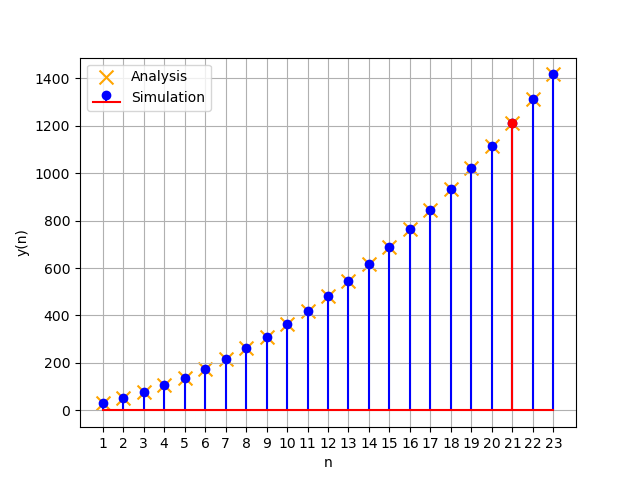
\includegraphics{figs/fig1.png}
    \caption{Six terms of given sequence}
    \label{fig:11_9_1_3 }
\end{figure}

\end{document}


\item If the sum of first 7 terms of an AP is 49 and that of 17 terms is 289, find the sum of first n terms.

\solution

\iffalse
\let\negmedspace\undefined
\let\negthickspace\undefined
\documentclass[journal,12pt,twocolumn]{IEEEtran}
\usepackage{cite}
\usepackage{amsmath,amssymb,amsfonts,amsthm}
\usepackage{algorithmic}
\usepackage{graphicx}
\usepackage{textcomp}
\usepackage{xcolor}
\usepackage{txfonts}
\usepackage{listings}
\usepackage{enumitem}
\usepackage{mathtools}
\usepackage{gensymb}
\usepackage{comment}
\usepackage[breaklinks=true]{hyperref}
\usepackage{tkz-euclide} 
\usepackage{listings}
\usepackage{gvv}                                        
\def\inputGnumericTable{}                                 
\usepackage[latin1]{inputenc}                                
\usepackage{color}                                            
\usepackage{array}                                            
\usepackage{longtable}                                       
\usepackage{calc}                                             
\usepackage{multirow}                                         
\usepackage{hhline}                                           
\usepackage{ifthen}                                           
\usepackage{lscape}
\newtheorem{theorem}{Theorem}[section]
\newtheorem{problem}{Problem}
\newtheorem{proposition}{Proposition}[section]
\newtheorem{lemma}{Lemma}[section]
\newtheorem{corollary}[theorem]{Corollary}
\newtheorem{example}{Example}[section]
\newtheorem{definition}[problem]{Definition}
\newcommand{\BEQA}{\begin{eqnarray}}
\newcommand{\EEQA}{\end{eqnarray}}
\newcommand{\define}{\stackrel{\triangle}{=}}
\theoremstyle{remark}
\newtheorem{rem}{Remark}
\begin{document}

\bibliographystyle{IEEEtran}
\vspace{3cm}

\title{10.5.3.9}
\author{EE23BTECH11063 - Vemula Siddhartha
}
\maketitle
\newpage
\bigskip

\renewcommand{\thefigure}{\theenumi}
\renewcommand{\thetable}{\theenumi}
\textbf{Question}:\\
If the sum of first 7 terms of an AP is 49 and that of 17 terms is 289, find the sum of
first n terms.
\\
\textbf{Solution: }
\fi
\begin{table}[h!]    
  \centering
  \begin{tabular}[12pt]{ |c| c|}
    \hline
    \textbf{Variable} & \textbf{Description}\\ 
    \hline
    $x\brak{0}$ & First term of the AP \\
    \hline 
    $d$ & Common difference of the AP\\
    \hline
    $y\brak{n}$ & Sum of $n+1$ terms of the AP\\
    \hline
    $x\brak{n}$ & General term\\
    \hline   
    \end{tabular}
  \caption{Variables Used}
  \label{tab10.5.3.9.1}
\end{table}
\begin{align}
y\brak{n}&=\frac{n+1}{2}\,\brak{2x\brak{0}+nd}\,u\brak{n}\label{eq10.5.3.9.1}\\
y\brak{6}&=49\\
y\brak{16}&=289
\end{align}
Then,
\begin{align}
x\brak{0}+3d&=7\label{eq10.5.3.9.2}\\
x\brak{0}+8d&=17 \label{eq10.5.3.9.3}
\end{align}
From  equations \ref{eq10.5.3.9.2} and \ref{eq10.5.3.9.3}, the augmented matrix is:
\begin{align}
 \myvec{
   1 & 3 & 7
   \\
   1 & 8 & 17
 }
 \xleftrightarrow[]{R_2 \leftarrow {R_2-R_1}}
 \myvec{
   1 & 3 & 7
   \\
   0 & 5 & 10
 }
 \\
 \xleftrightarrow[]{R_1 \leftarrow {R_1-\frac{3}{5}R_2}}
 \myvec{
   1 & 0 & 1
   \\
   0 & 5 & 10
 }
 \\
 \xleftrightarrow[]{R_2 \leftarrow \frac{R_2}{5}}
 \myvec{
   1 & 0 & 1
   \\
   0 & 1 & 2
 }
 \\
 \implies \myvec{
   x\brak{0}
   \\
   d
 }
 =
 \myvec{
   1
   \\
   2
 }
\end{align}
\begin{align}
    x\brak{n}&= \brak{1+2n}u\brak{n}\\
    X\brak{z}&=\frac{1}{1-z^{-1}}+\frac{2z^{-1}}{\brak{1-z^{-1}}^2}\;\;\cbrak{z\in\mathbb{C}: |z|>1}
\end{align}
\begin{align}
   y\brak{n}&=x\brak{n}*u\brak{n}\\
   Y\brak{z}&=X\brak{z}\,U\brak{z}\\
   \implies Y\brak{z}&=\brak{\frac{1}{1-z^{-1}}+\frac{2z^{-1}}{\brak{1-z^{-1}}^2}}\brak{\frac{1}{1-z^{-1}}}\\
   &=\frac{1}{\brak{1-z^{-1}}^2}+\frac{2z^{-1}}{\brak{1-z^{-1}}^3}\\
   \brak{n+1}u\brak{n}&\system{Z}\frac{1}{\brak{1-z^{-1}}^2}\cbrak{z\in\mathbb{C}: |z|>1}\\
   n\brak{\brak{n+1}u\brak{n}}&\system{Z}\frac{2z^{-1}}{\brak{1-z^{-1}}^3}\cbrak{z\in\mathbb{C}: |z|>1}
\end{align}
   From equations \eqref{eq:uzder-shift} and \eqref{eq:uzder-der}, taking the inverse Z Transform,
   \begin{align}
   y\brak{n}&=\brak{n+1}u\brak{n}+n\brak{\brak{n+1}u\brak{n}}\\
   \implies y\brak{n}&=\brak{n+1}^2\,u\brak{n}
\end{align}
\begin{figure}[h!]
   \centering
   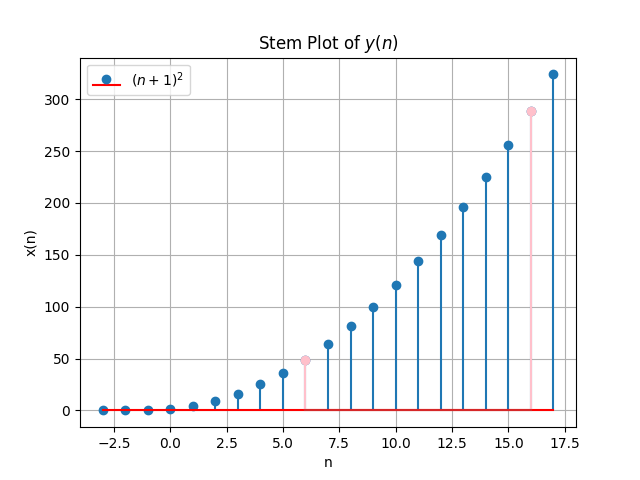
\includegraphics[width=1.1\linewidth]{ncert-maths/10/5/3/9/figs/Figure_1.png}
   \caption{Stem Plot of y\brak{n}}
   \label{stemplot}
\end{figure}  

\pagebreak

\item Write the first five terms of the sequence and obtain the corresponding series:\\
$a_1=a_2=2,$ $a_n=a_{n-1} -1,$ $n>2$\\
\solution
\iffalse
\let\negmedspace\undefined
\let\negthickspace\undefined
\documentclass[journal,12pt,twocolumn]{IEEEtran}
\usepackage{cite}
\usepackage{amsmath,amssymb,amsfonts,amsthm}
\usepackage{algorithmic}
\usepackage{graphicx}
\usepackage{textcomp}
\usepackage{xcolor}
\usepackage{txfonts}
\usepackage{listings}
\usepackage{enumitem}
\usepackage{mathtools}
\usepackage{float}
\usepackage{gensymb}
\usepackage{comment}
\usepackage[breaklinks=true]{hyperref}
\usepackage{tkz-euclide} 
\usepackage{listings}
\usepackage{gvv}                                        
\def\inputGnumericTable{}                                 
\usepackage[latin1]{inputenc}                                
\usepackage{color}                                            
\usepackage{array}                                            
\usepackage{longtable}                                       
\usepackage{calc}                                             
\usepackage{multirow}                                         
\usepackage{hhline}                                           
\usepackage{ifthen}                                           
\usepackage{lscape}
\usepackage{amsmath}
\newtheorem{theorem}{Theorem}[section]
\newtheorem{problem}{Problem}
\newtheorem{proposition}{Proposition}[section]
\newtheorem{lemma}{Lemma}[section]
\newtheorem{corollary}[theorem]{Corollary}
\newtheorem{example}{Example}[section]
\newtheorem{definition}[problem]{Definition}
\newcommand{\BEQA}{\begin{eqnarray}}
\newcommand{\EEQA}{\end{eqnarray}}
\newcommand{\define}{\stackrel{\triangle}{=}}
\theoremstyle{remark}
\newtheorem{rem}{Remark}
\begin{document}
\bibliographystyle{IEEEtran}
\title{NCERT 11.9.1.13Q}
\author{EE23BTECH11015 - DHANUSH V NAYAK$^{*}$% <-this % stops a space
}
\maketitle
\newpage
\bigskip
\renewcommand{\thefigure}{\arabic{figure}}
\renewcommand{\thetable}{\theenumi}
\textbf{Question:} Write the first five terms of each of the sequences in Exercises 11 to 13 and obtain the corresponding series:\\
$a_1=a_2=2,$\hspace{5pt} $a_n=a_{n-1} -1,$\hspace{5pt} $n>2$\\
\solution
\fi
\begin{table}[H]
    \centering
    \renewcommand\thetable{1}
    \setlength{\extrarowheight}{9pt}
    \resizebox{0.5\textwidth}{!}{
    \begin{tabular}{|c|c|c|}
    \hline
    \textbf{Parameter} & \textbf{Description} & \textbf{Value} \\ \hline
    $x\brak{0}$ & First term &2 \\ \hline
    $x\brak{1}$ & Second term &2 \\ \hline
    ROC & Region of convergence & $\left\{ z : \left|\sum_{n=-\infty}^{\infty} x(n)z^{-n}\right| < \infty \vphantom {\brak{{0.3pt}}}\right\}$ \\ \hline 
    $x(n)$ & General term & $x(n) = 
    \begin{cases}
        ? & ; n \geq 0 \\
        0 & ; n < 0 \\
    \end{cases}$ \\ \hline
    \end{tabular}}
    \caption{Parameter Table}
    \label{tab:11.9.1.13}
    \end{table}
\begin{align}
    x\brak{n} - x\brak{n-1} &= 2u\brak{n}-2u\brak{n-1}-u\brak{n-2}\label{eq:11.9.1.13.1}\\
X\brak{z}- z^{-1}X\brak{z} &= \frac{2}{\brak{1-z^{-1}}} - \frac{z^{-2}}{\brak{1-z^{-1}}}- \frac{2z^{-1}}{\brak{1-z^{-1}}}\\
    X\brak{z} &= \frac{2-2z^{-1}-z^{-2}}{\brak{1-z^{-1}}^2}  ,   \abs{z} >1
\end{align}
Using partial fractions
\begin{align}
    X\brak{z} &= \frac{2z^{-1}}{\brak{1-z^{-1}}} - \frac{z^{-2}}{\brak{1-z^{-1}}^2} + 2\label{eq:11.9.1.13.5}
\end{align}
Taking inverse $Z$-transform by result of equation \eqref{eq:11.9.5.26.9} in equation \eqref{eq:11.9.1.13.5}:
\begin{align}
    x\brak{n} &= 2u\brak{n}+\brak{1-n}u\brak{n-1}\label{eq:11.9.1.13.6}
\end{align}
\begin{figure}[H]
    \centering
    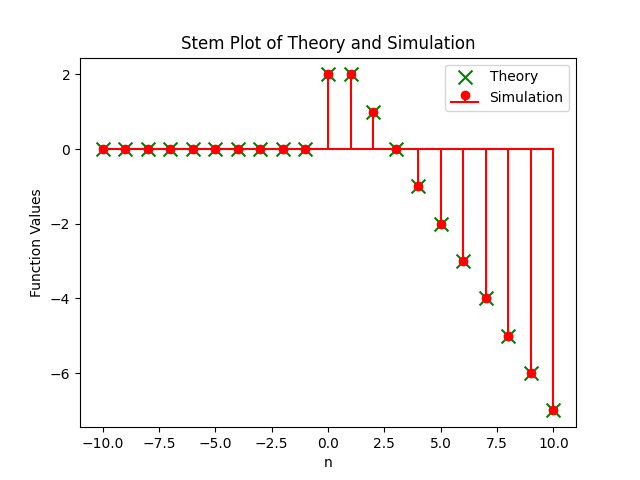
\includegraphics[width=1\columnwidth]{ncert-maths/11/9/1/13/figs/Theory_vs_Simulation.png}
    \caption{Comparison of Theory and Simulated Values}
    \label{fig:11.9.1.13.1}
\end{figure}
From the figure\figref{fig:11.9.1.13.1} we can see that the theoretical and simulated values overlap. 
%\end{document}

\pagebreak
\item Insert two numbers between 3 and 81 so that the resulting sequence is G.P.\\

\solution
\iffalse
\let\negmedspace\undefined
\let\negthickspace\undefined
\documentclass[journal,12pt,twocolumn]{IEEEtran}
\usepackage{cite}
\usepackage{amsmath,amssymb,amsfonts,amsthm}
\usepackage{algorithmic}
\usepackage{graphicx}
\usepackage{textcomp}
\usepackage{xcolor}
\usepackage{txfonts}
\usepackage{listings}
\usepackage{enumitem}
\usepackage{mathtools}
\usepackage{gensymb}
\usepackage{comment}
\usepackage[breaklinks=true]{hyperref}
\usepackage{tkz-euclide}
\usepackage{listings}
\usepackage{gvv}
\def\inputGnumericTable{}
\usepackage[latin1]{inputenc}
\usepackage{color}
\usepackage{array}
\usepackage{longtable}
\usepackage{calc}
\usepackage{multirow}
\usepackage{hhline}
\usepackage{ifthen}
\usepackage{lscape}

\newtheorem{theorem}{Theorem}[section]
\newtheorem{problem}{Problem}
\newtheorem{proposition}{Proposition}[section]
\newtheorem{lemma}{Lemma}[section]
\newtheorem{corollary}[theorem]{Corollary}
\newtheorem{example}{Example}[section]
\newtheorem{definition}[problem]{Definition}
\newcommand{\BEQA}{\begin{eqnarray}}
\newcommand{\EEQA}{\end{eqnarray}}
\newcommand{\define}{\stackrel{\triangle}{=}}
\theoremstyle{remark}
\newtheorem{rem}{Remark}
\begin{document}

\bibliographystyle{IEEEtran}
\vspace{3cm}

\title{NCERT Discrete 11.9.3 -26}
\author{EE23BTECH11057 - Shakunaveti Sai Sri Ram Varun$^{}$% &lt;-this % stops a space
}
\maketitle
\newpage
\bigskip
\vspace{2cm}
\textbf{Question: }
Insert two numbers between 3 and 81 so that the resulting sequence is G.P.\\
\textbf{Solution}:
\fi
\begin{table}[htbp] 
\centering
\begin{tabular}{|c|c|c|}
    \hline
    \textbf{Parameter} & \textbf{Description} & \textbf{Value} \\
    \hline
    $x\brak{0}$ & First term of G.P. & 3 \\
    \hline
    $x\brak{3}$ & Fourth term of G.P. & 81 \\
    \hline
    $r$ & common ratio of G.P. & r \\
    \hline
\end{tabular}



\caption{input values}
\label{tab: Table 11.9.3.26.15}
\end{table}
\begin{enumerate}
\item 
\begin{align}
x\brak{n}=x\brak{0}r^{n}
\end{align}
from the values in \tabref{tab: Table 11.9.3.26.15}
\begin{align}
%x(0)&=3\\
%x(3)&=81\\
\frac{x\brak{0}r^3}{x\brak{0}}&=27\\
r&=3
\end{align}
$ \therefore $ Required numbers are 9 and 27.
\item 
\begin{align}
x\brak{n} &= 3^{n+1}u\brak{n} \label{eq:11.9.3.26.1}\\
X\brak{z} &= \frac{3}{1-3z^{-1}} \quad |z|>3 \label{eq:11.9.3.26.2}
\end{align}
\begin{figure}[h!]
    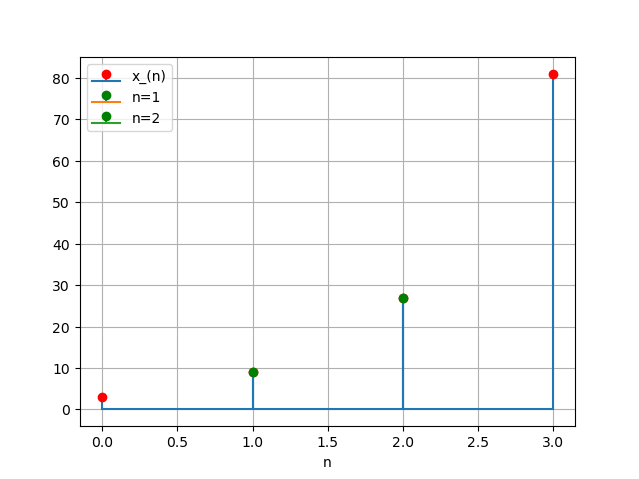
\includegraphics[width = \columnwidth]{ncert-maths/11/9/3/26/figs/Figure_1.png}
    \caption{Graph of $ x\brak{n}$ }
    \label{fig: 11.9.3.26.17}
\end{figure}
\end{enumerate}


\pagebreak

\item  What will Rs 500 amounts to in 10 years after its deposit in a bank which pays annual interest rate of 10$\%$ compounded annually?

\solution
    \let\negmedspace\undefined
\let\negthickspace\undefined
\documentclass[journal,12pt,twocolumn]{IEEEtran}
\usepackage{cite}
\usepackage{amsmath,amssymb,amsfonts,amsthm}
\usepackage{algorithmic}
\usepackage{graphicx}
\usepackage{textcomp}
\usepackage{xcolor}
\usepackage{txfonts}
\usepackage{listings}
\usepackage{enumitem}
\usepackage{mathtools}
\usepackage{gensymb}
\usepackage[breaklinks=true]{hyperref}
\usepackage{tkz-euclide} % loads  TikZ and tkz-base
\usepackage{listings}
\usepackage{gvv}


\newtheorem{theorem}{Theorem}[section]
\newtheorem{problem}{Problem}
\newtheorem{proposition}{Proposition}[section]
\newtheorem{lemma}{Lemma}[section]
\newtheorem{corollary}[theorem]{Corollary}
\newtheorem{example}{Example}[section]
\newtheorem{definition}[problem]{Definition}

\newcommand{\BEQA}{\begin{eqnarray}}
\newcommand{\EEQA}{\end{eqnarray}}
\newcommand{\define}{\stackrel{\triangle}{=}}
\theoremstyle{remark}
\newtheorem{rem}{Remark}

\graphicspath{./figs/}

%\bibliographystyle{ieeetr}
\begin{document}
%

\bibliographystyle{IEEEtran}


\vspace{3cm}

\title{
	%	\logo{
	Assignment-2

	\large{EE:1205 Signals and Systems}

	Indian Institute of Technology, Hyderabad
	%	}
}
\author{Kunal Thorawade

EE23BTECH11035
}	

\maketitle


\newpage

%\tableofcontents

\bigskip
 
 \renewcommand{\thefigure}{\theenumi}
 \renewcommand{\thetable}{\arabic{table}}
 %\renewcommand{\theequation}{\theenumi}

 \section{Question:}
 What will Rs 500 amounts to in 10 years after its deposit in a bank which pays annual interest rate of 10$\%$ compounded annually?

 \section{Solution}

 \begin{table}[ht]
    \centering
    \begin{tabular}{|c|c|c|}
        \hline
        Parameter & Value & Description \\
        \hline
        $x(0)$ & 5 & First term of AP \\
        $d$ & 1.75 & Common difference of AP \\
        $x(n)$ & 20.75 & $n^{th}$ term of AP \\
        \hline
    \end{tabular}
    \vspace{2mm}
    \caption{Parameter List}
    \label{tab:simple.10.5.2.20}
\end{table}


 The Z-transform of a sequence $x(n)$ is given by:

 \begin{align}
	     x(n) &= 500(1.1)^{n}u(n)
	       \\  X(Z) &= \frac{500}{1 - (1.1)z^{-1}} ; |z| > 1.1
 \end{align}

 \begin{figure}
	     \centering
	         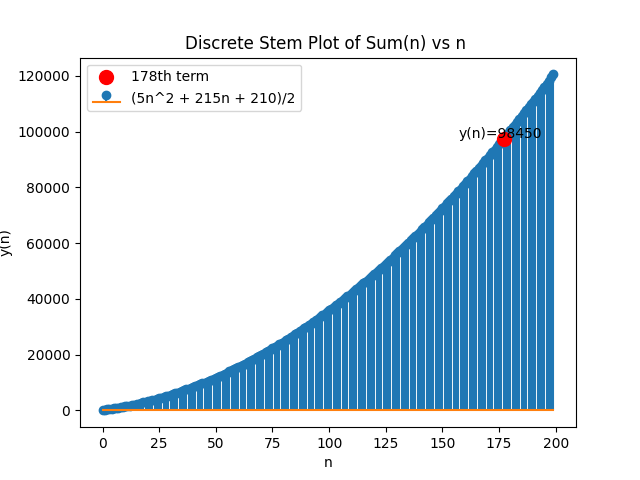
\includegraphics[width = 8cm]{figs/Fig1.png}
		     \caption{Plot of $x(n) = 500(1.1)^n$}
		         \label{fig:enter-label}
 \end{figure}
\end{document}

\pagebreak

\item Find the $20^{th}$ term from the last term of the AP: $3,8,13.....253$.

\solution
% \iffalse
\let\negmedspace\undefined
\let\negthickspace\undefined
\documentclass[journal,12pt,twocolumn]{IEEEtran}
\usepackage{cite}
\usepackage{amsmath,amssymb,amsfonts,amsthm}
\usepackage{algorithmic}
\usepackage{graphicx}
\usepackage{textcomp}
\usepackage{xcolor}
\usepackage{txfonts}
\usepackage{listings}
\usepackage{enumitem}
\usepackage{mathtools}
\usepackage{gensymb}
\usepackage{comment}
\usepackage[breaklinks=true]{hyperref}
\usepackage{tkz-euclide} 
\usepackage{listings}
\usepackage{gvv}                                        
\def\inputGnumericTable{}                                 
\usepackage[latin1]{inputenc}                                
\usepackage{color}                                            
\usepackage{array}                                            
\usepackage{longtable}                                       
\usepackage{calc}                                             
\usepackage{multirow}                                         
\usepackage{hhline}                                           
\usepackage{ifthen}                                           
\usepackage{lscape}
\usepackage{caption}
\newtheorem{theorem}{Theorem}[section]
\newtheorem{problem}{Problem}
\newtheorem{proposition}{Proposition}[section]
\newtheorem{lemma}{Lemma}[section]
\newtheorem{corollary}[theorem]{Corollary}
\newtheorem{example}{Example}[section]
\newtheorem{definition}[problem]{Definition}
\newcommand{\BEQA}{\begin{eqnarray}}
\newcommand{\EEQA}{\end{eqnarray}}
\newcommand{\define}{\stackrel{\triangle}{=}}
\theoremstyle{remark}
\newtheorem{rem}{Remark}
\begin{document}
\parindent 0px
\bibliographystyle{IEEEtran}
\vspace{3cm}

\title{NCERT 10.5.2 17Q}
\author{EE23BTECH11012 - Chavan Dinesh$^{*}$% <-this % stops a space
}
\maketitle
\newpage
\bigskip

\renewcommand{\thefigure}{\arabic{figure}}
\renewcommand{\thetable}{\arabic{table}}
\large\textbf{\textsl{Question:}}
Find the $20^{th}$ term from the last term of the AP: $3,8,13.....253$.

\solution

As the $20^{th}$ term is considered from last, 

\begin{table}[htbp]
    \centering
    \begin{table}[ht]
    \centering
    \begin{tabular}{|c|c|c|}
        \hline
        Parameter & Value & Description \\
        \hline
        $x(0)$ & 5 & First term of AP \\
        $d$ & 1.75 & Common difference of AP \\
        $x(n)$ & 20.75 & $n^{th}$ term of AP \\
        \hline
    \end{tabular}
    \vspace{2mm}
    \caption{Parameter List}
    \label{tab:simple.10.5.2.20}
\end{table}

    \caption{Input table}
    \label{tab:parameter_table.10.5.2.17}
\end{table}
% From \tabref{tab:parameter_table.10.5.2.17}:
% \begin{align}
%     x(n)&=x(0) + nd\\
%      x(19) &= 253 + (-5)19 \\
%         &= 158 
% \end{align}
% From \tabref{tab:parameter_table.10.5.2.17}:
% \begin{align}
% x(N-n)&=x(0) + (N-n)d\\
% x(N-19) &= 3 + (50 - 19)(5)\\
% &= 3 + 155\\
% &= 158
% \end{align}

From equation \eqref{eq:ztrans} and \eqref{eq:11.9.5.26.2}:
% \(Z\)-Transform of \(x(n)\):
\begin{align}
 X(z) =\frac{253}{1-z^{-1}}+ \frac{-5z^{-1}}{\brak{1-z^{-1}}^2};\cbrak{|z|>1}
\end{align}

\begin{figure}[ht]
    \centering
    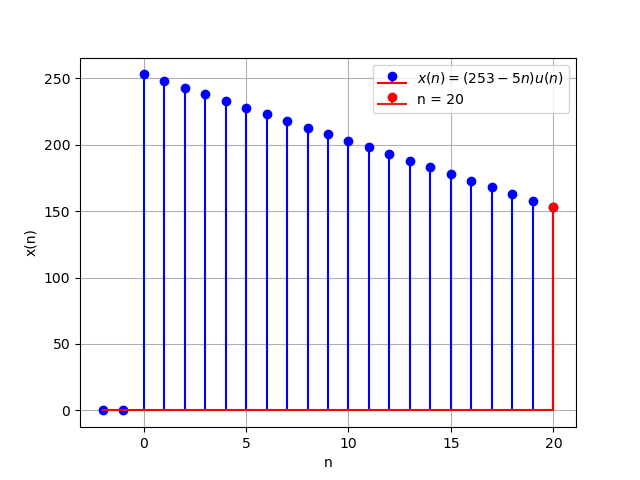
\includegraphics[width = \columnwidth]{figs/x(n)_vs_n.png}
    \caption{}
    \label{fig:graph1.10.5.2.17}
\end{figure}

\bibliographystyle{IEEEtran}
\end{document}


\pagebreak
\item Find the sum to $n$ terms of series , whose $n^{th}$ term is : $n(n+1)(n+4)$.

\solution
\iffalse
\documentclass[journal,12pt,twocolumn]{IEEEtran}
\usepackage{cite}
\usepackage{amsmath,amssymb,amsfonts,amsthm}
\usepackage{algorithmic}
\usepackage{graphicx}
\usepackage{textcomp}
\usepackage{xcolor}
\usepackage{txfonts}
\usepackage{listings}
\usepackage{enumitem}
\usepackage{mathtools}
\usepackage{gensymb}
\usepackage{comment}
\usepackage[breaklinks=true]{hyperref}
\usepackage{tkz-euclide}
\usepackage{listings}
\usepackage{gvv}
\def\inputGnumericTable{}
\usepackage[latin1]{inputenc}
\usepackage{color}
\usepackage{array}
\usepackage{longtable}
\usepackage{calc}
\usepackage{multirow}
\usepackage{hhline}
\usepackage{ifthen}
\usepackage{lscape}
\usepackage{caption}

\newtheorem{theorem}{Theorem}[section]
\newtheorem{problem}{Problem}
\newtheorem{proposition}{Proposition}[section]
\newtheorem{lemma}{Lemma}[section]
\newtheorem{corollary}[theorem]{Corollary}
\newtheorem{example}{Example}[section]
\newtheorem{definition}[problem]{Definition}
\newcommand{\BEQA}{\begin{eqnarray}}
\newcommand{\EEQA}{\end{eqnarray}}
\newcommand{\define}{\stackrel{\triangle}{=}}
\theoremstyle{remark}
\newtheorem{rem}{Remark}
\begin{document}

\bibliographystyle{IEEEtran}
\vspace{3cm}

\title{NCERT 11.9.4 8Q}
\author{EE23BTECH11010 - Venkatesh D Bandawar $^{*}$% <-this % stops a space
}
\maketitle
% \newpage
\bigskip

\renewcommand{\thefigure}{\theenumi}
\renewcommand{\thetable}{\theenumi}

\textbf{Question:} Find the sum to $n$ terms of series , whose $n^{th}$ term is : $n(n+1)(n+4)$.

\textbf{Solution}
\fi
\begin{table}[!h] 
\centering
\begin{tabular}{|c|c|c|}
\hline
\textbf{Parameter} & \textbf{Description} & \textbf{Value} \\
\hline
$x(n)$ & $n^{th}$ term of series & $n(n+1)(n+4)u(n)$\\
\hline
$y(n)$ & sum of n terms of series&\\
\hline
\end{tabular}

\caption{Given parameters}
\label{given parameters list.11.9.4.8}
\end{table}

\begin{align}
        n u(n) &\system{Z} \frac{z^{-1}}{\brak{1-z^{-1}}^2} \cbrak{\abs{z}>1} \label{eq:z transform of nu(n)} \\
        n^2 u(n) &\system{Z} \frac{z^{-1}\brak{1+z^{-1}}}{\brak{1-z^{-1}}^3} \cbrak{\abs{z}>1}\label{eq:z transform of n^2u(n)} \\
        n^3 u(n) &\system{Z} \frac{z^{-1}\brak{1+4z^{-1}+z^{-2}}}{\brak{1-z^{-1}}^4} \cbrak{\abs{z}>1}\label{eq:z transform of n^3u(n)} \\
        n^4 u(n) &\system{Z} \frac{z^{-1}\brak{1+11z^{-1}+11z^{-2}+z^{-3}}}{\brak{1-z^{-1}}^5} \cbrak{\abs{z}>1}\label{eq:z transform of n^4u(n)}
    \end{align}
From equation \eqref{eq:11.9.5.26.2} to \eqref{eq:11.9.5.26.4},\\
    \begin{multline}
        X(z) = \frac{z^{-1}\brak{1+4z^{-1}+z^{-2}}}{\brak{1-z^{-1}}^4} + \frac{5z^{-1}\brak{z^{-1}+1}}{\brak{1-z^{-1}}^3}\\ 
        + \frac{4z^{-1}}{\brak{1-z^{-1}}^2} \cbrak{\abs{z}>1}
    \end{multline}
    \begin{align}
         Y(z) &= X(z)U(z)\\
         &=\frac{z^{-1}\brak{1+4z^{-1}+z^{-2}}}{\brak{1-z^{-1}}^5} + \frac{5z^{-1}\brak{z^{-1}+1}}{\brak{1-z^{-1}}^4} + \frac{4z^{-1}}{\brak{1-z^{-1}}^3} 
    \end{align}
    \begin{multline}
        = \frac{1}{4}\sbrak{\frac{z^{-1}\brak{1+11z^{-1}+11z^{-2}+z^{-3}}}{\brak{1-z^{-1}}^5}} \\
        +\frac{13}{6}\sbrak{\frac{z^{-1}\brak{1+4z^{-1}+z^{-2}}}{\brak{1-z^{-1}}^4}} + \frac{19}{4}\sbrak{\frac{z^{-1}\brak{1+z^{-1}}}{\brak{1-z^{-1}}^3}}\\
        + \frac{17}{6}\sbrak{\frac{z^{-1}}{\brak{1-z^{-1}}^2}} \cbrak{\abs{z}>1}
    \end{multline}
    Taking reverse z transform, using equations \eqref{eq:z transform of nu(n)} to \eqref{eq:z transform of n^4u(n)}
    \begin{align}
        y(n) = \brak{\frac{n^4}{4} + \frac{13n^3}{6} + \frac{19n^2}{4} + \frac{17n}{6}} u\brak{n}
    \end{align}
    \begin{multline}
        = \brak{\frac{n^4}{4} + \frac{2n^3}{4} + \frac{10n^3}{6} + \frac{n^2}{4} + \frac{15n^2}{6} + \frac{4n^2}{2} + \frac{5n}{6} + \frac{4n}{2}} u\brak{n}
    \end{multline}
    \begin{multline}
        = \brak{\frac{n^4+2n^3+n^4}{4}}u\brak{n} +\brak{\frac{10n^3+15n^2+5n}{6}}u\brak{n}\\
        +\brak{\frac{4n^2+4n}{2}}u\brak{n}
    \end{multline}
    \begin{multline}
        = \brak{\frac{n^2\brak{n+1}^2}{4} + \frac{5n(n+1)(2n+1)}{6} 
        + \frac{4n(n+1)}{2}} u\brak{n}
    \end{multline}
    \begin{figure}[!h] 
    \centering
    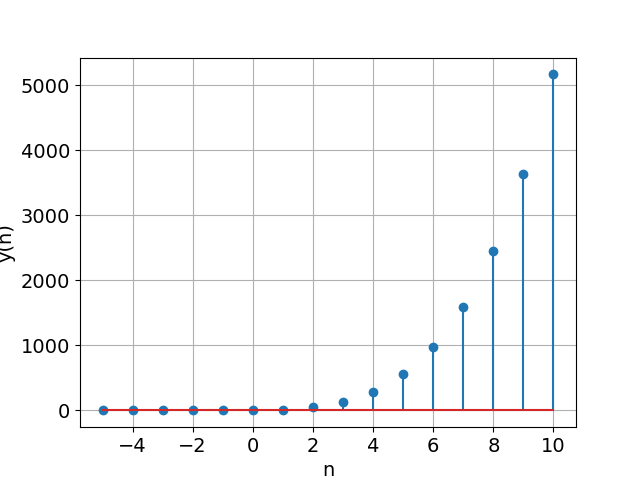
\includegraphics[width=\columnwidth]{ncert-maths/11/9/4/8/figs/sumplot.png}
    \caption{Sum of n terms of series}
    \label{fig:Graph1_math.11.9.4.8}
    \end{figure}


\pagebreak

\item Find the indicated terms in the sequence whose nth terms is $a(n)$ = $4n-3$. Find $a(17)$ and $a(24)$.
    
\solution 
\let\negmedspace\undefined
\let\negthickspace\undefined
\documentclass[journal,12pt,twocolumn]{IEEEtran}

\usepackage{cite}
\usepackage{amsmath,amssymb,amsfonts,amsthm}
\usepackage{algorithmic}
\usepackage{graphicx}
\usepackage{textcomp}
\usepackage{xcolor}
\usepackage{txfonts}
\usepackage{listings}
\usepackage{enumitem}
\usepackage{mathtools}
\usepackage{gensymb}
\usepackage[breaklinks=true]{hyperref}
\usepackage{tkz-euclide} % loads  TikZ and tkz-base
\usepackage{listings}
\usepackage{circuitikz}
\usepackage{graphicx}

%\newcounter{MYtempeqncnt}
\DeclareMathOperator*{\Res}{Res}
%\renewcommand{\baselinestretch}{2}
\renewcommand\thesection{\arabic{section}}
\renewcommand\thesubsection{\thesection.\arabic{subsection}}
\renewcommand\thesubsubsection{\thesubsection.\arabic{subsubsection}}

\renewcommand\thesectiondis{\arabic{section}}
\renewcommand\thesubsectiondis{\thesectiondis.\arabic{subsection}}
\renewcommand\thesubsubsectiondis{\thesubsectiondis.\arabic{subsubsection}}

% correct bad hyphenation here
\hyphenation{op-tical net-works semi-conduc-tor}
\def\inputGnumericTable{}                                 %%

\lstset{
	frame=single,
	breaklines=true,
	columns=fullflexible
}



\newtheorem{theorem}{Theorem}[section]
\newtheorem{problem}{Problem}
\newtheorem{proposition}{Proposition}[section]
\newtheorem{lemma}{Lemma}[section]
\newtheorem{corollary}[theorem]{Corollary}
\newtheorem{example}{Example}[section]
\newtheorem{definition}[problem]{Definition}
\newcommand{\BEQA}{\begin{eqnarray}}
	\newcommand{\EEQA}{\end{eqnarray}}
\newcommand{\define}{\stackrel{\triangle}{=}}
\newcommand\figref{Fig.~\ref}
\newcommand\tabref{Table~\ref}
\bibliographystyle{IEEEtran}
%\bibliographystyle{ieeetr}


\providecommand{\mbf}{\mathbf}
\providecommand{\pr}[1]{\ensuremath{\Pr\left(#1\right)}}
\providecommand{\qfunc}[1]{\ensuremath{Q\left(#1\right)}}
\providecommand{\sbrak}[1]{\ensuremath{{}\left[#1\right]}}
\providecommand{\lsbrak}[1]{\ensuremath{{}\left[#1\right.}}
\providecommand{\rsbrak}[1]{\ensuremath{{}\left.#1\right]}}
\providecommand{\brak}[1]{\ensuremath{\left(#1\right)}}
\providecommand{\lbrak}[1]{\ensuremath{\left(#1\right.}}
\providecommand{\rbrak}[1]{\ensuremath{\left.#1\right)}}
\providecommand{\cbrak}[1]{\ensuremath{\left\{#1\right\}}}
\providecommand{\lcbrak}[1]{\ensuremath{\left\{#1\right.}}
\providecommand{\rcbrak}[1]{\ensuremath{\left.#1\right\}}}
\theoremstyle{remark}
\newtheorem{rem}{Remark}
\newcommand{\sgn}{\mathop{\mathrm{sgn}}}
\providecommand{\abs}[1]{\left\vert#1\right\vert}
\providecommand{\res}[1]{\Res\displaylimits_{#1}}
\providecommand{\norm}[1]{\left\lVert#1\right\rVert}
%\providecommand{\norm}[1]{\lVert#1\rVert}
\providecommand{\mtx}[1]{\mathbf{#1}}
\providecommand{\mean}[1]{E\left[ #1 \right]}
\providecommand{\fourier}{\overset{\mathcal{F}}{ \rightleftharpoons}}
%\providecommand{\hilbert}{\overset{\mathcal{H}}{ \rightleftharpoons}}
\providecommand{\system}{\overset{\mathcal{H}}{ \longleftrightarrow}}
%\newcommand{\solution}[2]{\textbf{Solution:}{#1}}
\newcommand{\solution}{\noindent \textbf{Solution: }}
\newcommand{\cosec}{\,\text{cosec}\,}
\providecommand{\dec}[2]{\ensuremath{\overset{#1}{\underset{#2}{\gtrless}}}}
\newcommand{\myvec}[1]{\ensuremath{\begin{pmatrix}#1\end{pmatrix}}}
\newcommand{\mydet}[1]{\ensuremath{\begin{vmatrix}#1\end{vmatrix}}}
\renewcommand{\abstractname}{Question}

\let\vec\mathbf

	
	\vspace{3cm}
	
	


\newcommand{\permcomb}[4][0mu]{{{}^{#3}\mkern#1#2_{#4}}}
\newcommand{\comb}[1][-1mu]{\permcomb[#1]{C}}

%\IEEEpeerreviewmaketitle

\newcommand \tab [1][1cm]{\hspace*{#1}}
%\newcommand{\Var}{$\sigma ^2$}
\usepackage{amssymb}
\usepackage{amsmath}
\title{
	
\title{NCERT Discrete 11.9.1 Q7}
\author{EE23BTECH11061 - SWATHI DEEPIKA$^{*}$% <-this % stops a space
}


}
\begin{document}

\maketitle

\textbf{Question:} 
Find the indicated terms in the sequence whose nth terms is $a(n)$ = $4n-3$. Find $a(17)$ and $a(24)$.
    
\solution
In the question, following information is provided:
 
 \begin{table}[h]
 	\centering
 	\resizebox{6 cm}{!}{
 		\begin{table}[ht]
    \centering
    \begin{tabular}{|c|c|c|}
        \hline
        Parameter & Value & Description \\
        \hline
        $x(0)$ & 5 & First term of AP \\
        $d$ & 1.75 & Common difference of AP \\
        $x(n)$ & 20.75 & $n^{th}$ term of AP \\
        \hline
    \end{tabular}
    \vspace{2mm}
    \caption{Parameter List}
    \label{tab:simple.10.5.2.20}
\end{table}

 	}
 	\vspace{6 pt}
 	\caption{Parameters}
 	\label{tab:sw_tabel} 
 \end{table}

\begin{align}
x(n) = (4n+1)(u(n))
\end{align}

\begin{align}
 x(16) = 4 \times 16 + 1 = 65
\end{align}

\begin{align}
x(23) = 4 \times 23 + 1 = 93
\end{align}

Using Z-Transform,
\begin{align}
X(z) = 4\frac{z^{-1}}{(1-z^{-1})^2} + \frac{1}{1-z^{-1}}
 \quad |z| > 1
\end{align}

\begin{figure}[!h]
    \centering
    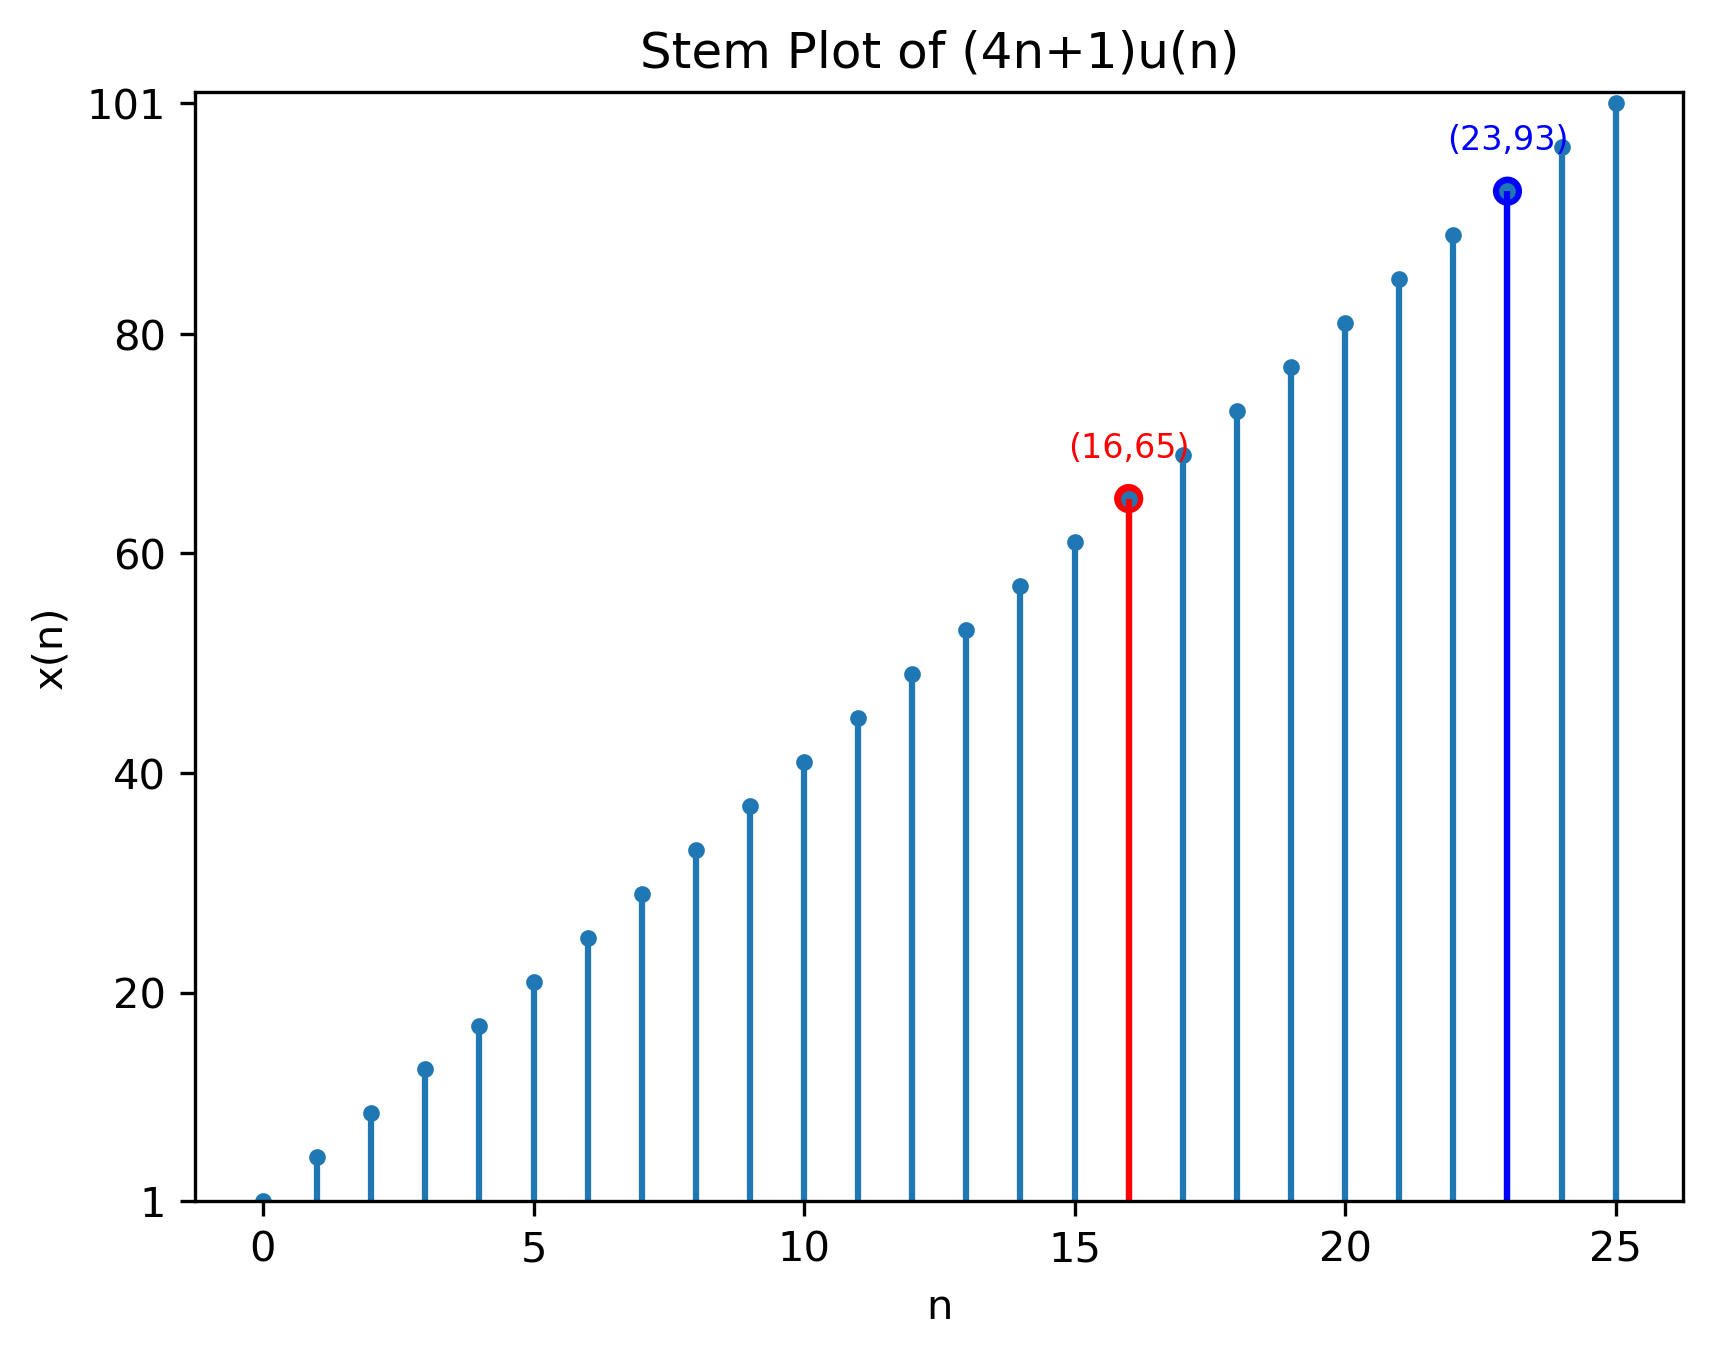
\includegraphics[width = \columnwidth]{figs/a_plot.png}
    \caption{$x(n)$ vs $n$}
    \label{fig:sw_plot}
\end{figure}



\end{document}




\pagebreak

\item The difference between any two cosecutive interior angles of a polygon is $5^\circ$.If the smallest angle is $120^\circ$,find the number of sides of polygon. \\
\solution
\iffalse
\let\negmedspace\undefined
\let\negthickspace\undefined
\documentclass[journal,12pt,twocolumn]{IEEEtran}
\usepackage{cite}
\usepackage{amsmath,amssymb,amsfonts,amsthm}
%\usepackage{algorithmic}
\usepackage{graphicx}
\usepackage{textcomp}
\usepackage{xcolor}
\usepackage{txfonts}
\usepackage{listings}
\usepackage{enumitem}
\usepackage{mathtools}
\usepackage{gensymb}
\usepackage{comment}
\usepackage[breaklinks=true]{hyperref}
\usepackage{tkz-euclide} % loads  TikZ and tkz-base
\usepackage{listings}
\usepackage[latin1]{inputenc}                                
\usepackage{color}                                            
\usepackage{array}                                            
\usepackage{longtable}                                       
\usepackage{calc}                                             
\usepackage{multirow}                                         
\usepackage{hhline}                                           
\usepackage{ifthen}                                           
\usepackage{lscape}
\usepackage{caption}
\usepackage{gvv}

\newtheorem{theorem}{Theorem}[section]
\newtheorem{problem}{Problem}
\newtheorem{proposition}{Proposition}[section]
\newtheorem{lemma}{Lemma}[section]
\newtheorem{corollary}[theorem]{Corollary}
\newtheorem{example}{Example}[section]
\newtheorem{definition}[problem]{Definition}
%\newtheorem{thm}{Theorem}[section] 
%\newtheorem{defn}[thm]{Definition}
%\newtheorem{algorithm}{Algorithm}[section]
%\newtheorem{cor}{Corollary}
\newcommand{\BEQA}{\begin{eqnarray}}
\newcommand{\system}[1]{\stackrel{#1}{\rightarrow}}
\newcommand{\EEQA}{\end{eqnarray}}
\newcommand{\define}{\stackrel{\triangle}{=}}
\theoremstyle{remark}
\newtheorem{rem}{Remark}
%\bibliographystyle{ieeetr}

\begin{document}
\providecommand{\pr}[1]{\ensuremath{\Pr\left(#1\right)}}
\providecommand{\prt}[2]{\ensuremath{p_{#1}^{\left(#2\right)} }}        % own macro for this question
\providecommand{\qfunc}[1]{\ensuremath{Q\left(#1\right)}}
\providecommand{\sbrak}[1]{\ensuremath{{}\left[#1\right]}}
\providecommand{\lsbrak}[1]{\ensuremath{{}\left[#1\right.}}
\providecommand{\rsbrak}[1]{\ensuremath{{}\left.#1\right]}}
\providecommand{\brak}[1]{\ensuremath{\left(#1\right)}}
\providecommand{\lbrak}[1]{\ensuremath{\left(#1\right.}}
\providecommand{\rbrak}[1]{\ensuremath{\left.#1\right)}}
\providecommand{\cbrak}[1]{\ensuremath{\left\{#1\right\}}}
\providecommand{\lcbrak}[1]{\ensuremath{\left\{#1\right.}}
\providecommand{\rcbrak}[1]{\ensuremath{\left.#1\right\}}}
\newcommand{\sgn}{\mathop{\mathrm{sgn}}}
\providecommand{\abs}[1]{\left\vert#1\right\vert}
\providecommand{\res}[1]{\Res\displaylimits_{#1}} 
\providecommand{\norm}[1]{\left\lVert#1\right\rVert}
%\providecommand{\norm}[1]{\lVert#1\rVert}
\providecommand{\mtx}[1]{\mathbf{#1}}
\providecommand{\mean}[1]{E\left[ #1 \right]}
\providecommand{\cond}[2]{#1\middle|#2}
\providecommand{\fourier}{\overset{\mathcal{F}}{ \rightleftharpoons}}
\newenvironment{amatrix}[1]{%
  \left(\begin{array}{@{}*{#1}{c}|c@{}}
}{%
  \end{array}\right)
}
%\providecommand{\hilbert}{\overset{\mathcal{H}}{ \rightleftharpoons}}
%\providecommand{\system}{\overset{\mathcal{H}}{ \longleftrightarrow}}
        %\newcommand{\solution}[2]{\textbf{Solution:}{#1}}
\newcommand{\solution}{\noindent \textbf{Solution: }}
\newcommand{\cosec}{\,\text{cosec}\,}
\providecommand{\dec}[2]{\ensuremath{\overset{#1}{\underset{#2}{\gtrless}}}}
\newcommand{\myvec}[1]{\ensuremath{\begin{pmatrix}#1\end{pmatrix}}}
\newcommand{\mydet}[1]{\ensuremath{\begin{vmatrix}#1\end{vmatrix}}}
\newcommand{\myaugvec}[2]{\ensuremath{\begin{amatrix}{#1}#2\end{amatrix}}}
\providecommand{\rank}{\text{rank}}
\providecommand{\pr}[1]{\ensuremath{\Pr\left(#1\right)}}
\providecommand{\qfunc}[1]{\ensuremath{Q\left(#1\right)}}
        \newcommand*{\permcomb}[4][0mu]{{{}^{#3}\mkern#1#2_{#4}}}
\newcommand*{\perm}[1][-3mu]{\permcomb[#1]{P}}
\newcommand*{\comb}[1][-1mu]{\permcomb[#1]{C}}
\providecommand{\qfunc}[1]{\ensuremath{Q\left(#1\right)}}
\providecommand{\gauss}[2]{\mathcal{N}\ensuremath{\left(#1,#2\right)}}
\providecommand{\diff}[2]{\ensuremath{\frac{d{#1}}{d{#2}}}}
\providecommand{\myceil}[1]{\left \lceil #1 \right \rceil }
\newcommand\figref{Fig.~\ref}
\newcommand\tabref{Table~\ref}
\newcommand{\sinc}{\,\text{sinc}\,}
\newcommand{\rect}{\,\text{rect}\,}
%%
%       %\newcommand{\solution}[2]{\textbf{Solution:}{#1}}
%\newcommand{\solution}{\noindent \textbf{Solution: }}
%\newcommand{\cosec}{\,\text{cosec}\,}
%\numberwithin{equation}{section}
%\numberwithin{equation}{subsection}
%\numberwithin{problem}{section}
%\numberwithin{definition}{section}
%\makeatletter
%\@addtoreset{figure}{problem}
%\makeatother

%\let\StandardTheFigure\thefigure
\let\vec\mathbf

\bibliographystyle{IEEEtran}

\vspace{3cm}
\title{Assignment}
\author{EE23BTECH11008 - Meenakshi}
\maketitle
\newpage
\bigskip

\renewcommand{\thefigure}{\theenumi}
\renewcommand{\thetable}{\theenumi}
%\renewcommand{\theequation}{\theenumi}
Q:The difference between any two cosecutive interior angles of a polygon is $5^\circ$.If the smallest angle is $120^\circ$,find the number of sides of polygon. \\
\solution
\fi
\begin{table}[!ht]
    \centering
         \begin{tabular}{|c|c|c|} 
      \hline
\textbf{Variable}& \textbf{Description}& \textbf{Value}\\\hline
$x(0)$& first term of AP& 120  \\\hline
    d& common difference of AP & 5\\\hline
    $x(n)$ & general  term of AP&none\\\hline
\end{tabular}

    \caption{input parameters}
    \label{tab:11_9_2_1}
\end{table}

Sum of interior angles of a polygon with $n+1$ sides is given by
\begin{align}
    S &= (n-1)180
\end{align}
Sum of $n$ terms of AP is given by
\begin{align}
    y(n) &= x(n)*u(n)
\end{align}
where $x(n) = 120 + 5n$
\begin{equation}
    x(n)*u(n)=(n-1)180 \label{eq:11.9.2.4.eq}
\end{equation}
\begin{align}
    Y(z) &= X(z)U(z) \\
    &= \left(\frac{x(0)}{1-z^{-1}} + \frac{dz^{-1}}{(1-z^{-1})^2}\right) \frac{1}{1-z^{-1}} \quad |z|>1\\
    &=\frac{120}{(1-z^{-1})^2} + \frac{5z^{-1}}{(1-z^{-1})^3} \quad |z|>1
\end{align}
\begin{align}
	\brak{n+1}u\brak{n}&\system{ Z}\left(\frac{1}{\brak{1-z^{-1}}^2}\right)\quad |z|>1\label{eq:11.9.2.18.9} \\
	\frac{\brak{n}\brak{n-1}}{2}u\brak{n-1} &\system{Z}\left(\frac{z^{-1}}{\brak{1-z^{-1}}^3}\right) \quad |z|>1\label{eq:11.9.2.18.10}
\end{align}
applying inverse Z-transform for each term and solving we get,
\begin{align}
    y\brak{n} &= \frac{n+1}{2}\brak{240+5n}u(n)
\end{align}
now from ~\eqref{eq:11.9.2.4.eq} 
\begin{align}
y(n) &= (n-1)180 \\
\frac{n+1}{2}\brak{240+5n}u(n) &= (n-1)180
\end{align}
now replace $n$ by $n-1$: 
\begin{align}
    n(235+5n) &= (n-2)360\\
    5n^2-125n+720 &= 0
\end{align}
\begin{align}
   n &= 16,9
\end{align}

\begin{figure}[h]
\centering
 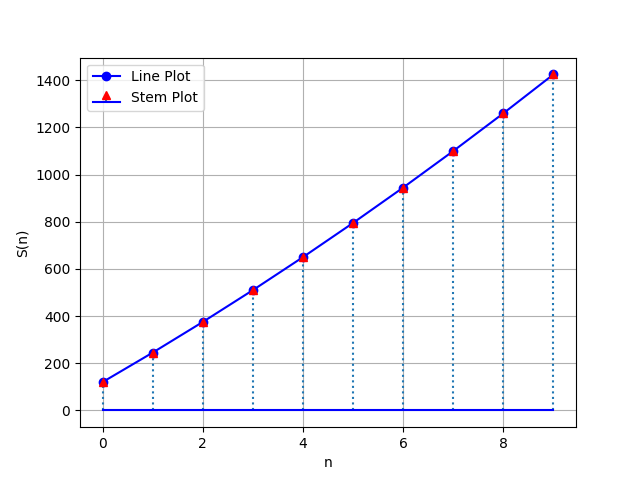
\includegraphics[width=\columnwidth]{ncert-maths/11/9/2/18/figs/python.1(1).png} 
  \captionsetup{justification=centering}
  \caption{Plot of the sum of n terms taken from Python}
  \label{fig:your_label}
\end{figure}

%\end{document}
   
   




\pagebreak
\item The $5$th,$8$th and $11$th terms of a GP are p,q and s respectively .show that $q^2=ps$ \\
\solution
\iffalse
\let\negmedspace\undefined
\let\negthickspace\undefined
\documentclass[journal,12pt,twocolumn]{IEEEtran}
\usepackage{cite}
\usepackage{amsmath,amssymb,amsfonts,amsthm}
\usepackage{algorithmic}
\usepackage{graphicx}
\usepackage{textcomp}
\usepackage{xcolor}
\usepackage{txfonts}
\usepackage{listings}
\usepackage{enumitem}
\usepackage{mathtools}
\usepackage{gensymb}
\usepackage{comment}
\usepackage[breaklinks=true]{hyperref}
\usepackage{tkz-euclide} 
\usepackage{listings}
\usepackage{gvv}                                        
\def\inputGnumericTable{}                                 
\usepackage[latin1]{inputenc}                                
\usepackage{color}                                            
\usepackage{array}                                            
\usepackage{longtable}                                       
\usepackage{calc}                                             
\usepackage{multirow}                                         
\usepackage{hhline}                                           
\usepackage{ifthen}                                           
\usepackage{lscape}

\newtheorem{theorem}{Theorem}[section]
\newtheorem{problem}{Problem}
\newtheorem{proposition}{Proposition}[section]
\newtheorem{lemma}{Lemma}[section]
\newtheorem{corollary}[theorem]{Corollary}
\newtheorem{example}{Example}[section]
\newtheorem{definition}[problem]{Definition}
\newcommand{\BEQA}{\begin{eqnarray}}
\newcommand{\EEQA}{\end{eqnarray}}
\newcommand{\define}{\stackrel{\triangle}{=}}
\theoremstyle{remark}
\newtheorem{rem}{Remark}
\begin{document}

\bibliographystyle{IEEEtran}
\vspace{3cm}

\title{11.9.3.3}
\author{EE23BTECH11065 - prem sagar}
\maketitle
\newpage

\bigskip 

\renewcommand{\thefigure}{\theenumi}
\renewcommand{\thetable}{\theenumi}
\textbf{Question}:\\ The $5$th,$8$th and $11$th terms of a GP are p,q and s respectively .show that $q^2=ps$
\\\\\textbf{solution}:
\fi
\begin{table}[!ht]
   \centering
    \renewcommand\thetable{1}
      \begin{tabular}{|c|c|c|}
    \hline
            \textbf{Symbol} & \textbf{Value} & \textbf{Description} \\
    \hline
          $x\brak{5}$ & $p$ & $x\brak{0}r^5$ \\
    \hline
          $x\brak{8}$ & $q$ & $x\brak{0}r^8$\\
    \hline 
          $x\brak{{11}}$ &$s$ &$x\brak{0}r^{11}$ \\
    \hline
          $x\brak{n}$ & &$x\brak{0}r^nu\brak{n}$ \\
    \hline
          $r$& $\brak{\frac{s}{p}}^\frac{1}{6}$& common ratio\\
     \hline     
  \end{tabular}

    \caption{input parameters}
    \label{tab:11.9.3}
 \end{table}
\\ From \tabref{tab:11.9.3}:
\begin{align}
q^2&=x\brak{0}\,r^8\,x\brak{0}\,r^8
     \\ &=x\brak{0}^2\,r^{16}
\\ps&=x\brak{0}\,r^5\,x(0)\,r^{11}
       \\&=x\brak{0}^2\,r^{16}
\\\implies q^2&=ps
\end{align}
now we will find r and x\brak{0}:
\begin{align}
\frac{s}{p}&=\frac{x\brak{0}r^{11}}{x\brak{0}r^5}
\\r&=\brak{\frac{s}{p}}^\frac{1}{6} 
\\p&=x\brak{0}\brak{\frac{s}{p}}^\frac{5}{6}
\\x\brak{0}&=\frac{p^\frac{11}{6}}{s^\frac{5}{6}}
\end{align}
Applying z-Transform:
\begin{align}
     X(z) &= \frac{x\brak{0}}{1-r\,z^{-1}}\: \:,\abs{z}>\abs{r}
\\ \implies  X(z)&=\frac{p^3}{p^\frac{7}{6}s^\frac{5}{6}-q^2z^{-1}}\:,\abs{z}>\abs{\brak{\frac{q}{p}}^\frac{1}{3}}
     \end{align}    
\\\begin{figure}[h]
   \renewcommand\thefigure{1}
    \centering
    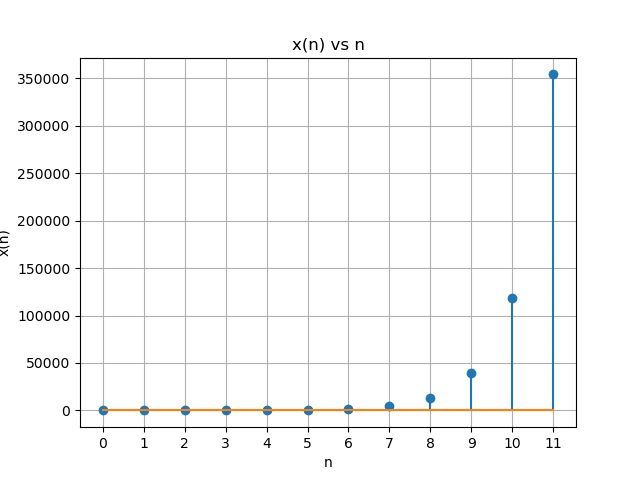
\includegraphics[width=1\linewidth]{/root/assign1/figs/figure__plot.png}
    \caption{plot x\brak{n}vs n\hspace{0.1cm}$p=486$,
    \hspace{0.1cm}$q=13122$,
    \hspace{0.1cm}$s=354294$,
    \hspace{0.1cm}$r=3$}
    \label{fig:1}
\end{figure}\\
\end{document}

\pagebreak
\item The sum of the first four terms of an A.P. is 56. The sum of the last four terms is
 112. If its first term is 11, then find the number of terms.\\
\solution
\iffalse
\let\negmedspace\undefined
\let\negthickspace\undefined
\documentclass[journal,12pt,twocolumn]{IEEEtran}
\usepackage{cite}
\usepackage{amsmath,amssymb,amsfonts,amsthm}
\usepackage{algorithmic}
\usepackage{graphicx}
\usepackage{textcomp}
\usepackage{xcolor}
\usepackage{txfonts}
\usepackage{listings}
\usepackage{enumitem}
\usepackage{mathtools}
\usepackage{gensymb}
\usepackage{comment}
\usepackage[breaklinks=true]{hyperref}
\usepackage{tkz-euclide} 
\use-package{listings}
\usepackage{gvv}                                        
\def\inputGnumericTable{}                                 
\usepackage[latin1]{inputenc}                                
\usepackage{color}                                            
\usepackage{array}                                            
\usepackage{longtable}                                       
\usepackage{calc}                                             
\usepackage{multirow}                                         
\usepackage{hhline}                                           
\usepackage{ifthen}                                           
\usepackage{lscape}
\usepackage{caption}

\newtheorem{theorem}{Theorem}[section]
\newtheorem{problem}{Problem}
\newtheorem{proposition}{Proposition}[section]
\newtheorem{lemma}{Lemma}[section]
\newtheorem{corollary}[theorem]{Corollary}
\newtheorem{example}{Example}[section]
\newtheorem{definition}[problem]{Definition}
\newcommand{\BEQA}{\begin{eqnarray}}
\newcommand{\EEQA}{\end{eqnarray}}
\newcommand{\define}{\stackrel{\triangle}{=}}
\theoremstyle{remark}
\newtheorem{rem}{Remark}
\begin{document}

\bibliographystyle{IEEEtran}
\vspace{3cm}

\title{11.9.5}
\author{EE23BTECH11029 - Kanishk}
\maketitle

\bigskip


\textbf{Question}:\\ 
The sum of the first four terms of an A.P. is 56. The sum of the last four terms is
112. If its first term is 11, then find the number of terms.\\

\textbf{Solution}:\\ 
\fi
\begin{table}[ht]
    \centering
    \def\arraystretch{1.5}
    \footnotesize
\begin{tabular}{|c|c|c|}
\hline
Symbol & Value & Description\\
\hline
$x(0)$ & $11$ & First term of AP \\
\hline
$y\brak{3}$ & $56$ & Sum of the first four terms of AP\\
\hline
$y\brak{n}-y\brak{n-4}$ & $112$& Sum of the last four terms of AP\\
\hline
\end{tabular}

   \caption{Input Parameters}
   \label{tab:11.9.5.12}
\end{table}

\small
\begin{align}
y\brak{n}&=\sbrak{\frac{\brak{n+1}}{2}\brak{2x\brak{0}+nd}}u\brak{n}\\
\implies y(3)&=\frac{4}{2}\brak{2x\brak{0}+3d}\\
\end{align}
From \tabref{tab:11.9.5.12}:
\begin{align}
\frac{4}{2}\brak{2x\brak{0}+3d}&=56\\
2x\brak{0}+3d&=28\\
\implies d&=2
\end{align}

\begin{align}
 y\brak{n}-y\brak{n-4}&=\frac{4}{2}\brak{2x\brak{n}+3\brak{-d}}
\end{align}
From \tabref{tab:11.9.5.12}:
\begin{align}
\frac{4}{2}\brak{2x\brak{n}+3\brak{-d}}&=112\\
2x\brak{n}-3d&=56\\
\implies x\brak{n}&=31\\
x\brak{0}+\brak{n}2&=31\\
\implies n&=10
\end{align}


\begin{align}
x\brak{n}&=\brak{x\brak{0}+2n}u\brak{n}\\
\implies X\brak{z}&=\frac{x\brak{0}}{1-z^{-1}}+2\frac{z^{-1}}{\brak{1-z^{-1}}^{2}}.\quad \abs{z} > 1
\end{align}

\newpage

\begin{figure}
    
    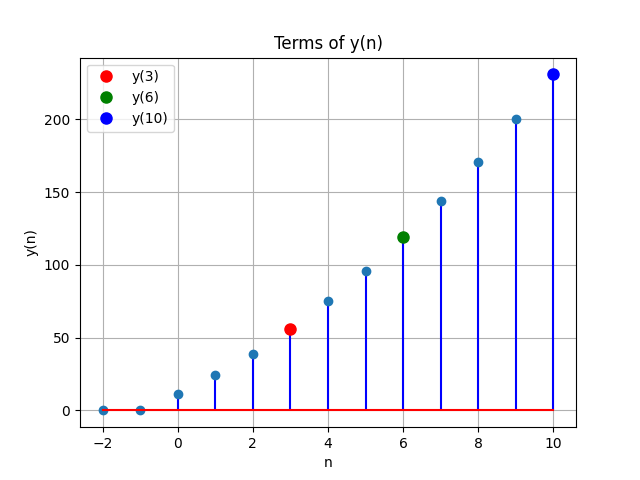
\includegraphics[width=\columnwidth]{ncert-maths/11/9/5/12//figs/fig1.png}
    \caption{Plot y(n) vs n}
\end{figure}

%\end{document}
\pagebreak
\item Find a GP for which sum of the first two terms is -4 and the fifth term is 4 times the third term.
\solution
\iffalse
\let\negmedspace\undefined
\let\negthickspace\undefined
\documentclass[journal,12pt,twocolumn]{IEEEtran}
\usepackage{cite}
\usepackage{amsmath,amssymb,amsfonts,amsthm}
\usepackage{algorithmic}
\usepackage{graphicx}
\usepackage{textcomp}
\usepackage{xcolor}
\usepackage{txfonts}
\usepackage{listings}
\usepackage{enumitem}
\usepackage{mathtools}
\usepackage{gensymb}
\usepackage{comment}
\usepackage[breaklinks=true]{hyperref}
\usepackage{tkz-euclide} % loads  TikZ and tkz-base
\usepackage{listings}
\usepackage[latin1]{inputenc}                                
\usepackage{color}                                            
\usepackage{array}                                            
\usepackage{longtable}                                       
\usepackage{calc}                                             
\usepackage{multirow}                                         
\usepackage{hhline}                                           
\usepackage{ifthen}                                           
\usepackage{lscape}
\usepackage{caption}
\usepackage{subcaption}


\newtheorem{theorem}{Theorem}[section]
\newtheorem{problem}{Problem}
\newtheorem{proposition}{Proposition}[section]
\newtheorem{lemma}{Lemma}[section]
\newtheorem{corollary}[theorem]{Corollary}
\newtheorem{example}{Example}[section]
\newtheorem{definition}[problem]{Definition}
%\newtheorem{thm}{Theorem}[section] 
%\newtheorem{defn}[thm]{Definition}
%\newtheorem{algorithm}{Algorithm}[section]
%\newtheorem{cor}{Corollary}
\newcommand{\BEQA}{\begin{eqnarray}}
\newcommand{\EEQA}{\end{eqnarray}}
\newcommand{\define}{\stackrel{\triangle}{=}}
\theoremstyle{remark}
\newtheorem{rem}{Remark}
%\bibliographystyle{ieeetr}

\begin{document}

%
\providecommand{\pr}[1]{\ensuremath{\Pr\left(#1\right)}}
\providecommand{\prt}[2]{\ensuremath{p_{#1}^{\left(#2\right)} }}        % own macro for this question
\providecommand{\qfunc}[1]{\ensuremath{Q\left(#1\right)}}
\providecommand{\sbrak}[1]{\ensuremath{{}\left[#1\right]}}
\providecommand{\lsbrak}[1]{\ensuremath{{}\left[#1\right.}}
\providecommand{\rsbrak}[1]{\ensuremath{{}\left.#1\right]}}
\providecommand{\brak}[1]{\ensuremath{\left(#1\right)}}
\providecommand{\lbrak}[1]{\ensuremath{\left(#1\right.}}
\providecommand{\rbrak}[1]{\ensuremath{\left.#1\right)}}
\providecommand{\cbrak}[1]{\ensuremath{\left\{#1\right\}}}
\providecommand{\lcbrak}[1]{\ensuremath{\left\{#1\right.}}
\providecommand{\rcbrak}[1]{\ensuremath{\left.#1\right\}}}
\newcommand{\sgn}{\mathop{\mathrm{sgn}}}
\providecommand{\abs}[1]{\left\vert#1\right\vert}
\providecommand{\res}[1]{\Res\displaylimits_{#1}} 
\providecommand{\norm}[1]{\left\lVert#1\right\rVert}
%\providecommand{\norm}[1]{\lVert#1\rVert}
\providecommand{\mtx}[1]{\mathbf{#1}}
\providecommand{\mean}[1]{E\left[ #1 \right]}
\providecommand{\cond}[2]{#1\middle|#2}
\providecommand{\fourier}{\overset{\mathcal{F}}{ \rightleftharpoons}}
\newenvironment{amatrix}[1]{%
  \left(\begin{array}{@{}*{#1}{c}|c@{}}
}{%
  \end{array}\right)
}
%\providecommand{\hilbert}{\overset{\mathcal{H}}{ \rightleftharpoons}}
%\providecommand{\system}{\overset{\mathcal{H}}{ \longleftrightarrow}}
        %\newcommand{\solution}[2]{\textbf{Solution:}{#1}}
\newcommand{\solution}{\noindent \textbf{Solution: }}
\newcommand{\cosec}{\,\text{cosec}\,}
\providecommand{\dec}[2]{\ensuremath{\overset{#1}{\underset{#2}{\gtrless}}}}
\newcommand{\myvec}[1]{\ensuremath{\begin{pmatrix}#1\end{pmatrix}}}
\newcommand{\mydet}[1]{\ensuremath{\begin{vmatrix}#1\end{vmatrix}}}
\newcommand{\myaugvec}[2]{\ensuremath{\begin{amatrix}{#1}#2\end{amatrix}}}
\providecommand{\rank}{\text{rank}}
\providecommand{\pr}[1]{\ensuremath{\Pr\left(#1\right)}}
\providecommand{\qfunc}[1]{\ensuremath{Q\left(#1\right)}}
        \newcommand*{\permcomb}[4][0mu]{{{}^{#3}\mkern#1#2_{#4}}}
\newcommand*{\perm}[1][-3mu]{\permcomb[#1]{P}}
\newcommand*{\comb}[1][-1mu]{\permcomb[#1]{C}}
\providecommand{\qfunc}[1]{\ensuremath{Q\left(#1\right)}}
\providecommand{\gauss}[2]{\mathcal{N}\ensuremath{\left(#1,#2\right)}}
\providecommand{\diff}[2]{\ensuremath{\frac{d{#1}}{d{#2}}}}
\providecommand{\myceil}[1]{\left \lceil #1 \right \rceil }
\newcommand\figref{Fig.~\ref}
\newcommand\tabref{Table~\ref}
\newcommand{\sinc}{\,\text{sinc}\,}
\newcommand{\rect}{\,\text{rect}\,}
%%
%       %\newcommand{\solution}[2]{\textbf{Solution:}{#1}}
%\newcommand{\solution}{\noindent \textbf{Solution: }}
%\newcommand{\cosec}{\,\text{cosec}\,}
%\numberwithin{equation}{section}
%\numberwithin{equation}{subsection}
%\numberwithin{problem}{section}
%\numberwithin{definition}{section}
%\makeatletter
%\@addtoreset{figure}{problem}
%\makeatother

%\let\StandardTheFigure\thefigure
\let\vec\mathbf

\bibliographystyle{IEEEtran}

\vspace{3cm}
\title{Assignment}
\author{EE23BTECH11001 - Aashna Sahu}
\maketitle
\bigskip

\renewcommand{\thefigure}{\theenumi}
\renewcommand{\thetable}{\theenumi}
%\renewcommand{\theequation}{\theenumi}
Q:Find a GP for which sum of the first two terms is -4 and the fifth term is 4 times the third term.

\solution
\fi

\begin{table}[ht]
  \centering
  \begin{tabular}{|c|c|c|}
      \hline
      Parameter & Description & Value\\\hline
      $x(0)$ & First term of AP & --\\\hline
      $r$ & Common ratio & --\\\hline
      $x(n)$ & General term of given AP & $x(0)r^nu(n)$\\\hline
      $x(0)+x(1)$ & sum of 1st and 2nd term & $-4$\\\hline
      $\displaystyle\frac{x(4)}{x(2)}$ & Ratio of 5th and 3rd term & $4$\\\hline
\end{tabular}

  \caption{Input Parameters}
  \label{tab:table1}
\end{table}
From \tabref{tab:table1}:
\begin{align}
x(0)r^4&=4x(0)r^2\\
\implies r&=\pm 2
\label{eq:eq2}
\end{align}

From \tabref{tab:table1} and \eqref{eq:eq2} :\\
\begin{align}
x(0)r+x(0)&=-4\\
\implies x(0)&=\frac{-4}{r+1}\\
x(0) &=
\begin{cases}
   \displaystyle\frac{-4}{3}  , & r=+2 \\
      4  , & r=-2 \\
\end{cases}\\
   X(z)&=\frac{x(0)}{1-rz^{-1}}\quad ,\abs{z}>\abs{r}\\
X(z) &=
\begin{cases}
   \displaystyle\frac{4}{3(2z^{-1}-1)}, & r=+2\\
   \displaystyle\frac{4}{1+2z^{-1}}, & r=-2\\
\end{cases}
\end{align}

\[\abs{z}>2\]

\begin{figure}[h]
  \centering
  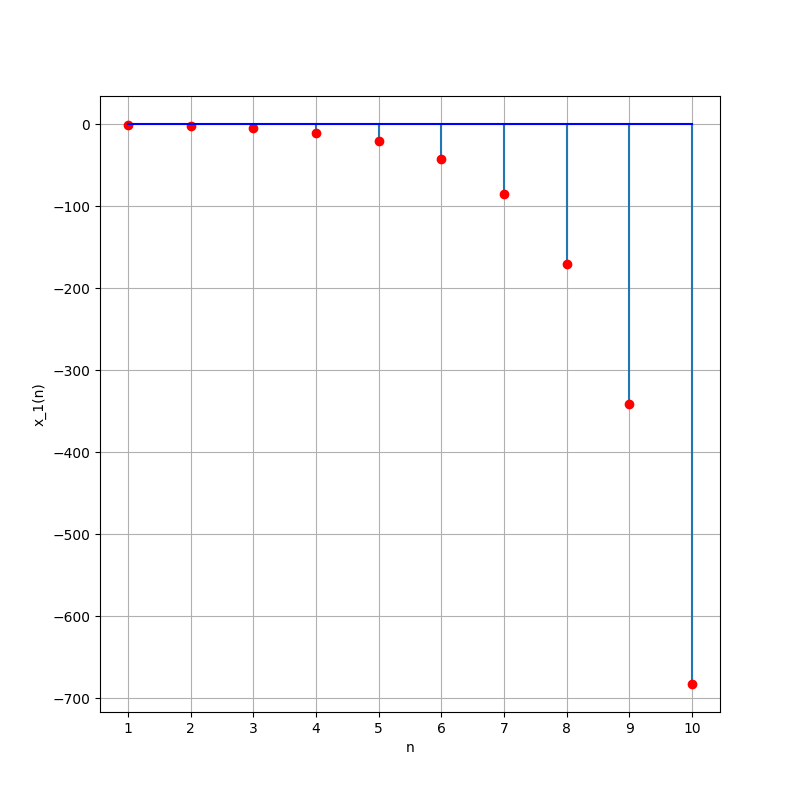
\includegraphics[width=1.0\columnwidth]{ncert-maths/11/9/3/16/figs/plot1.png}
  \caption{Representation of x(n) for $r=2$}
  \label{fig:fig1}
\end{figure}
\begin{figure}[h]
  \centering
  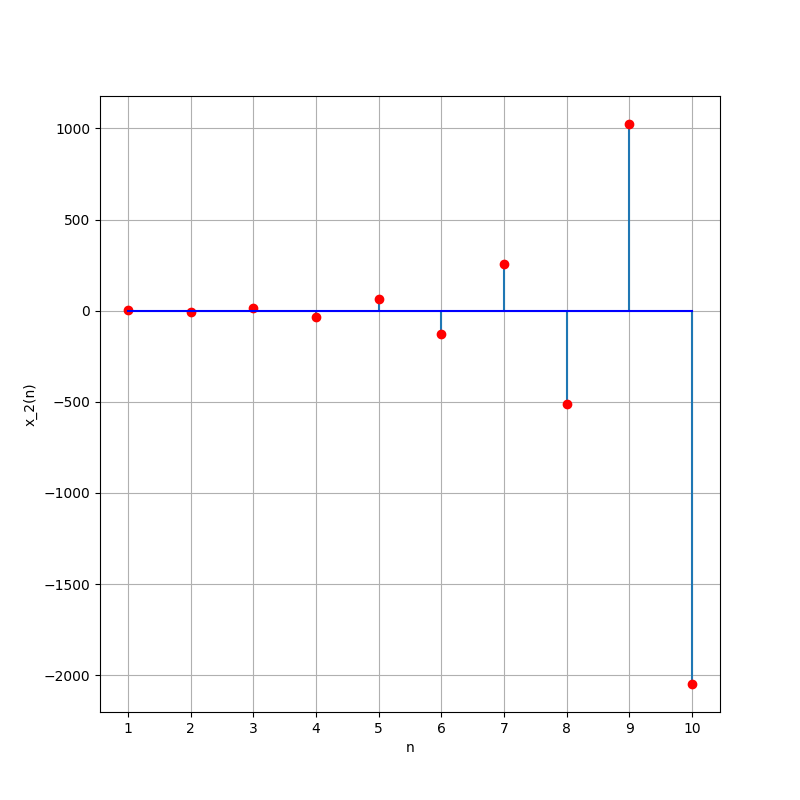
\includegraphics[width=1.0\columnwidth]{ncert-maths/11/9/3/16/figs/plot2.png}
  \caption{Representation of x(n) for $r=-2$}
  \label{fig:fig2}
\end{figure}


%\end{document}

\pagebreak
\end{enumerate}
